%Version 3.1 December 2024
% See section 11 of the User Manual for version history
%
%%%%%%%%%%%%%%%%%%%%%%%%%%%%%%%%%%%%%%%%%%%%%%%%%%%%%%%%%%%%%%%%%%%%%%
%%                                                                 %%
%% Please do not use \input{...} to include other tex files.       %%
%% Submit your LaTeX manuscript as one .tex document.              %%
%%                                                                 %%
%% All additional figures and files should be attached             %%
%% separately and not embedded in the \TeX\ document itself.       %%
%%                                                                 %%
%%%%%%%%%%%%%%%%%%%%%%%%%%%%%%%%%%%%%%%%%%%%%%%%%%%%%%%%%%%%%%%%%%%%%

%%\documentclass[referee,sn-basic]{sn-jnl}% referee option is meant for double line spacing

%%=======================================================%%
%% to print line numbers in the margin use lineno option %%
%%=======================================================%%

%%\documentclass[lineno,pdflatex,sn-basic]{sn-jnl}% Basic Springer Nature Reference Style/Chemistry Reference Style

%%=========================================================================================%%
%% the documentclass is set to pdflatex as default. You can delete it if not appropriate.  %%
%%=========================================================================================%%

%%\documentclass[sn-basic]{sn-jnl}% Basic Springer Nature Reference Style/Chemistry Reference Style

%%Note: the following reference styles support Namedate and Numbered referencing. By default the style follows the most common style. To switch between the options you can add or remove “Numbered” in the optional parenthesis. 
%%The option is available for: sn-basic.bst, sn-chicago.bst%  
 
%%\documentclass[pdflatex,sn-nature]{sn-jnl}% Style for submissions to Nature Portfolio journals
%%\documentclass[pdflatex,sn-basic]{sn-jnl}% Basic Springer Nature Reference Style/Chemistry Reference Style
\documentclass[pdflatex,sn-mathphys-num]{sn-jnl}% Math and Physical Sciences Numbered Reference Style
%%\documentclass[pdflatex,sn-mathphys-ay]{sn-jnl}% Math and Physical Sciences Author Year Reference Style
%%\documentclass[pdflatex,sn-aps]{sn-jnl}% American Physical Society (APS) Reference Style
%%\documentclass[pdflatex,sn-vancouver-num]{sn-jnl}% Vancouver Numbered Reference Style
%%\documentclass[pdflatex,sn-vancouver-ay]{sn-jnl}% Vancouver Author Year Reference Style
%%\documentclass[pdflatex,sn-apa]{sn-jnl}% APA Reference Style
%%\documentclass[pdflatex,sn-chicago]{sn-jnl}% Chicago-based Humanities Reference Style

%%%% Standard Packages
%%<additional latex packages if required can be included here>

\usepackage{graphicx}%
\usepackage{multirow}%
\usepackage{amsmath,amssymb,amsfonts}%
\usepackage{amsthm}%
\usepackage{mathrsfs}%
\usepackage[title]{appendix}%
\usepackage{xcolor}%
\usepackage{textcomp}%
\usepackage{manyfoot}%
\usepackage{booktabs}%
\usepackage{algorithm}%
\usepackage{algorithmicx}%
\usepackage{algpseudocode}%
\usepackage{listings}%
\usepackage{placeins}%
%%%%

%%%%%=============================================================================%%%%
%%%%  Remarks: This template is provided to aid authors with the preparation
%%%%  of original research articles intended for submission to journals published 
%%%%  by Springer Nature. The guidance has been prepared in partnership with 
%%%%  production teams to conform to Springer Nature technical requirements. 
%%%%  Editorial and presentation requirements differ among journal portfolios and 
%%%%  research disciplines. You may find sections in this template are irrelevant 
%%%%  to your work and are empowered to omit any such section if allowed by the 
%%%%  journal you intend to submit to. The submission guidelines and policies 
%%%%  of the journal take precedence. A detailed User Manual is available in the 
%%%%  template package for technical guidance.
%%%%%=============================================================================%%%%

%% as per the requirement new theorem styles can be included as shown below
\theoremstyle{thmstyleone}%
\newtheorem{theorem}{Theorem}%  meant for continuous numbers
%%\newtheorem{theorem}{Theorem}[section]% meant for sectionwise numbers
%% optional argument [theorem] produces theorem numbering sequence instead of independent numbers for Proposition
\newtheorem{proposition}[theorem]{Proposition}% 
\newtheorem{lemma}[theorem]{Lemma}%
\newtheorem{corollary}[theorem]{Corollary}%
%%\newtheorem{proposition}{Proposition}% to get separate numbers for theorem and proposition etc.

\theoremstyle{thmstyletwo}%
\newtheorem{example}{Example}%
\newtheorem{remark}{Remark}%

\theoremstyle{thmstylethree}%
\newtheorem{definition}{Definition}%

\raggedbottom
%%\unnumbered% uncomment this for unnumbered level heads

\begin{document}

\newcommand{\pepfigure}[3]{\begin{figure}[t]\centering
\IfFileExists{figures/#1.pdf}{\includegraphics[width=\textwidth]{figures/#1.pdf}}{\fbox{\parbox{0.9\textwidth}{\centering figure \detokenize{#1} not generated yet}}}
\caption{#2}\label{#3}\end{figure}}

\title[PEP-AI Validated Quantization]{PEP-AI Validated Quantization for Energy-Efficient Perception in Intelligent Transportation Systems}

\author*[1]{\fnm{Tamás} \sur{Menyhárt}}\email{menyhart.tamas@inf.unideb.hu}
\author[1]{\fnm{András} \sur{Hajdu}}\email{hajdu.andras@inf.unideb.hu}
\author[1]{\fnm{Róbert} \sur{Lakatos}}\email{lakatos.robert@inf.unideb.hu}

\affil*[1]{\orgdiv{Department of Data Science and Visualization, Faculty of Informatics}, \orgname{University of Debrecen}, \orgaddress{\city{Debrecen}, \country{Hungary}}}

\abstract{\textbf{Background:} Post-training INT8 quantization reduces the inference energy of camera-based perception, but quantized models are accepted on output-level accuracy, which does not show where the quantization error arises, how it propagates and when it causes detection errors.

\textbf{Methods:} Five detection and classification networks were compiled into strict-FP32, FP16, INT8 and FP8 TensorRT engines on an NVIDIA H200. We prove a rounding-noise lemma and propagation bounds for the relative error, test them on layer-wise activations, relate the local deviation to detection errors, and measure latency, energy and robustness under eight adverse conditions.

\textbf{Results:} INT8 was 1.6--11.8$\times$ faster than FP32 and 1.1--1.5$\times$ faster than FP16 and used 72--91\% less energy per image; FP16 was lossless and FP8 lost at most 0.4 points, INT8 between 0.25 mAP and 41 top-1 points. The noise of each INT8 quantizer was predicted within 1.1--2.8\,dB, FP32 statistics alone screened the networks, and one measurement of the quantized head input predicted the relative INT8 loss within a factor of about two (tenfold per 12\,dB, Spearman $\rho=1.0$, $n=5$). The fragile networks also lost up to 36\% under low contrast and up to 17 points depending on the order of the calibration images; FP8 did not. Each doubling of the local deviation raised the odds of a vanishing detection 1.7--4.2-fold.

\textbf{Conclusion:} The error of a quantized network is predictable from FP32 statistics up to a measurable propagation factor, which identifies the networks for which INT8 is safe; for a 1\,000-vehicle fleet the measured INT8 saving is up to 1\,GWh and 251\,t CO$_2$ per year.}

\keywords{post-training quantization, INT8, FP8, TensorRT, energy efficiency, explainable AI, sustainable AI, intelligent transportation systems}

\maketitle

\section{Introduction}\label{sec:intro}

Camera-based perception runs continuously on every camera stream of an automated vehicle, so that its energy scales with fleet size, frame rate and operating hours~\cite{veres2020deep}; at wide adoption the emissions of onboard computing could approach those of today's data centres~\cite{sudhakar2023datacenters}. The energy of machine learning is a recognised sustainability problem~\cite{strubell2019energy,schwartz2020green,wu2022sustainable,lannelongue2021green}, inference dominates it for many deployed models~\cite{luccioni2024power,desislavov2023trends}, and reported savings should be measured rather than estimated~\cite{henderson2020reporting}. For transport, the European Green Deal requires a 90\% cut of emissions by 2050 while automated mobility is to be deployed at scale~\cite{ec2019greendeal,ec2020mobility}. The choice of a numerical format is therefore a trade-off between energy cost, emissions and perception errors. In AI-based business optimisation (AIBO), model outputs enter managerial decisions whose cost includes both operating expenses and the consequences of errors~\cite{duan2019decision}; for quantization this requires the measured energy per inference and the error rate relative to the reference model, which aggregate accuracy does not provide.

Post-training quantization (PTQ) maps weights and activations from 32-bit floating point (FP32) to 8-bit integers (INT8) without retraining~\cite{jacob2018quantization,krishnamoorthi2018whitepaper,nagel2021whitepaper,gholami2021survey}. It reduces memory traffic fourfold, and an 8-bit integer multiplication or addition costs 18--30 times less energy than its FP32 counterpart~\cite{horowitz2014energy}. On a GPU these savings require integer kernels generated by an inference compiler~\cite{wu2020integer,tensorrt}; quantization simulated in floating point yields none. Research on PTQ minimises the output error of the quantized model: adaptive rounding~\cite{nagel2020adaround}, layer-wise optimisation on small calibration sets~\cite{hubara2021accurate} and block reconstruction~\cite{li2021brecq,wei2022qdrop} optimise the rounding of weights, cross-layer equalisation balances per-channel ranges~\cite{nagel2019datafree}, outlier channel splitting reduces clipping~\cite{zhao2019ocs}, and mixed-precision methods allocate bit widths from second-order sensitivities~\cite{dong2019hawq,yao2021hawqv3}.

Analytical models treat the rounding error of a single quantizer as additive noise, uniform within the clipping range; this model underlies analytical range setting~\cite{banner2019aciq,nagel2021whitepaper} and the comparison of integer and floating-point formats~\cite{kuzmin2022fp8,vanbaalen2023fp8}. How the noise of many quantizers combines through a nonlinear network has been bounded under distributional assumptions~\cite{sakr2017analytical} or controlled by non-expansive layers~\cite{lin2019defensive}, but not decomposed into quantities that can be estimated from FP32 statistics and tested on a deployed engine. Such a decomposition would predict, before deployment, which networks tolerate INT8 and which layers must stay in higher precision.

PTQ methods are evaluated by aggregate accuracy, which can remain stable while internal representations change and compressed models disagree on a subset of inputs~\cite{hooker2019forget}. Aggregate accuracy does not show where the error arises, whether it predicts the errors that matter, or how it behaves under distribution shift, all of which safety standards for road vehicles require to be analysed~\cite{iso21448,iso8800,mohseni2022taxonomy}. Depthwise-separable networks are sensitive to per-tensor activation quantization~\cite{sheng2018quantization,wu2020integer}, and quantized classifiers are more sensitive to natural corruptions such as fog or blur~\cite{xiao2023robustness,michaelis2019benchmarking,zhang2023adverse}; for detectors on integer kernels, the link between the per-layer error and detection failures has not been quantified.

Our conference paper introduced the Precise, Explainable and Provable (PEP-AI) framework for activation-level validation of quantized networks~\cite{menyhart2026citds}: the median relative error of channel-projected activations, symmetric-logarithmic hexbin densities and an attenuation model of layer-wise error propagation. It analysed one backbone in simulated INT8 with qualitative failure examples; deployed integer engines, further architectures and a quantitative link between the deviation and detection errors were left open. This article extends it as follows:
\begin{itemize}
\item \emph{Theory:} a rounding-noise lemma for INT8 and floating-point formats, a corollary for static scales, an additive decomposition of the head-input error over the quantizers and a bound for contracting chains, with proofs and quantitative tests (Sections~\ref{sec:noise} and~\ref{sec:propagation}).
\item \emph{Measurement:} strict-FP32, FP16, INT8 and FP8 TensorRT engines of five networks on an H200, with accuracy and paired bootstrap intervals, latency, jitter, memory traffic and energy.
\item \emph{Validation:} a detection-level test of the deviation--error link, robustness under eight adverse conditions, and two INT8 failure modes that aggregate accuracy does not reveal: dependence on the order of the calibration images and broken duplicate suppression in an NMS-free detector.
\item \emph{Prediction:} a five-step procedure that screens a network for INT8 from FP32 statistics and, after one measurement of the quantized head input, predicts its relative accuracy loss, worked through and checked against the measurements for every step (Section~\ref{sec:worked}).
\item \emph{Decision:} a fleet cost model with a break-even penalty per quantization-induced error.
\end{itemize}
Proofs, implementation details and supplementary analyses are in Appendices~\ref{sec:supp-methods} and~\ref{sec:supp-results}, extended tables and figures in Appendix~\ref{secA1}.

\section{Methods}\label{sec:methods}

\subsection{PEP-AI validation pipeline}\label{sec:pipeline}

PEP-AI compares the activations of a quantized network with those of its FP32 reference. \emph{Precise}: per-tensor, per-image deviation statistics of every analysed layer of the deployed engine. \emph{Explainable}: an analytical model of where the deviation is injected and how it propagates, supported by activation maps and density plots. \emph{Provable}: statements proved under explicit assumptions (Lemma~\ref{lem:noise}, Corollary~\ref{cor:static}, Propositions~\ref{prop:selective} and~\ref{prop:fixedpoint}) and empirical claims with a stated sample and uncertainty. The pipeline (Fig.~\ref{fig:pipeline}) exports each FP32 model to ONNX, quantizes it into explicit quantize--dequantize (QDQ) graphs, compiles strongly typed TensorRT engines and measures accuracy, activation deviation, the deviation--error link, latency, energy and robustness; the layer-level diagnosis feeds back into quantization. All stages are scripted and seeded and regenerate every number, figure and table.

\begin{figure}[t]
\centering
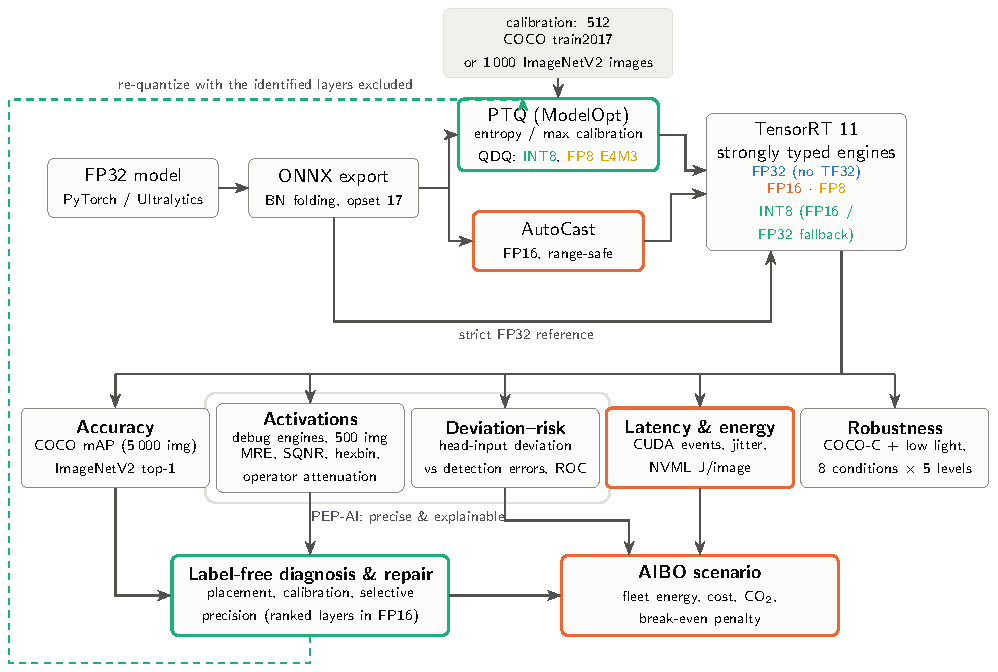
\includegraphics[width=\textwidth]{figures/fig_pipeline.pdf}
\caption{PEP-AI validation pipeline. The FP32 model is exported once and turned into an FP16 variant and into INT8 and FP8 variants that share one calibration; every variant is compiled into a strongly typed TensorRT engine and evaluated along five measurement branches. The activation analysis feeds back into quantization (label-free diagnosis and repair, dashed), and the measured energy, accuracy and error rates feed the AIBO scenario.}\label{fig:pipeline}
\end{figure}

\subsection{Models and data}\label{sec:models}

Five convolutional architectures covering two-stage detection, one-stage detection and classification were evaluated (Table~\ref{tab:models}): Faster R-CNN with a ResNet-50 FPN backbone~\cite{ren2017faster} (torchvision COCO weights, frozen batch normalisation folded into the convolutions before export), YOLOv10-S and YOLOv10-X~\cite{wang2024yolov10} with their NMS-free one-to-one head, and EfficientNet-B0~\cite{tan2019efficientnet} and DenseNet-121~\cite{huang2017densely} (torchvision ImageNet weights).

% BEGIN GENERATED M1_models
\begin{table}[h]
\footnotesize\setlength{\tabcolsep}{4pt}
\caption{Evaluated architectures}\label{tab:models}
\begin{tabular}{@{}lllrrrrrr@{}}
\toprule
Model & Task & Input & Params (M) & GFLOPs & Convs & \multicolumn{3}{c}{Weights (MB)} \\
\cmidrule{7-9}
 & & & & & & FP32 & FP16 & INT8 \\
\midrule
Faster R-CNN R50-FPN & det. & 800$\times$1088 & 26.8 & 240.4 & 61 & 107.3 & 53.7 & 27.0 \\
YOLOv10-S & det. & 640$\times$640 & 8.1 & 24.9 & 86 & 29.0 & 14.5 & 7.4 \\
YOLOv10-X & det. & 640$\times$640 & 31.8 & 170.8 & 174 & 117.9 & 58.9 & 29.9 \\
EfficientNet-B0 & cls. & 224$\times$224 & 5.3 & 0.8 & 81 & 21.1 & 10.5 & 6.8 \\
DenseNet-121 & cls. & 224$\times$224 & 8.0 & 5.7 & 120 & 32.2 & 16.1 & 9.3 \\
\botrule
\end{tabular}
\footnotetext{Faster R-CNN: backbone and FPN only (the part that is quantized); GFLOPs at the benchmark input size. INT8 weight size counts quantized weights at 1 byte and the remaining tensors in FP16.}
\end{table}
% END GENERATED M1_models

Detectors were evaluated on the complete COCO 2017 validation split (5\,000 images)~\cite{lin2014microsoft}; the activation analysis and the robustness study use the first 500 images of a seeded permutation of it. Calibration used 512 seeded images from the COCO 2017 \emph{training} split, so that calibration and evaluation data are disjoint. The classifiers were evaluated on ImageNetV2 (matched frequency)~\cite{recht2019imagenet}, split with a fixed seed into 1\,000 calibration and 9\,000 evaluation images. Pre-processing follows each model's reference implementation (Table~\ref{tab:datasets}); about 40\% of all COCO objects belong to traffic-relevant categories.

% BEGIN GENERATED M2_datasets
\begin{table}[h]
\footnotesize\setlength{\tabcolsep}{4pt}
\caption{Data splits}\label{tab:datasets}
\begin{tabular}{@{}llrrrrr@{}}
\toprule
Split & Purpose & Images & Objects & Obj./img & S/M/L (\%) & Traffic (\%) \\
\midrule
train2017 subset & calibration (detectors) & 512 & 3\,401 & 6.6 & 43 / 32 / 25 & 44 \\
val2017 & mAP, deviation--risk & 5\,000 & 36\,335 & 7.3 & 42 / 34 / 24 & 41 \\
val2017 first 500 & activations, robustness & 500 & 3\,787 & 7.6 & 44 / 33 / 23 & 41 \\
INV2 calibration & calibration (classifiers) & 1\,000 & -- & -- & -- & -- \\
INV2 evaluation & top-1, activations & 9\,000 & -- & -- & -- & -- \\
\botrule
\end{tabular}
\footnotetext{Traffic: share of objects in the classes person, bicycle, car, motorcycle, bus, truck, traffic light and stop sign. S/M/L: COCO size classes by box area ($<32^2$, $32^2$--$96^2$, $>96^2$ pixels). All subsets are drawn with a fixed seed.}
\end{table}
% END GENERATED M2_datasets

\subsection{Quantization and deployment}\label{sec:quant}

Post-training quantization used NVIDIA TensorRT Model Optimizer~\cite{modelopt} without fine-tuning~\cite{jacob2018quantization,krishnamoorthi2018whitepaper,nagel2021whitepaper}. For a tensor $x$ and a scale $s>0$, the symmetric INT8 quantizer is
\begin{equation}
Q_s(x)=s\cdot\operatorname{clip}\!\left(\lfloor x/s\rceil,-127,127\right),\label{eq:int8}
\end{equation}
with one scale per output channel for weights and one scale $s=\alpha/127$ per tensor for activations. The clipping range $\alpha$ is set on the calibration images by entropy calibration~\cite{migacz2017tensorrt} (Eq.~\eqref{eq:entropy}) or, as an ablation, by the observed maximum; the sensitivity of the result to the calibration sample, which matters for small calibration sets~\cite{hubara2021accurate}, was measured by recalibrating every model on seeded random subsets of its calibration set and, as a control, with an order-independent implementation of entropy calibration (Supplementary Section~\ref{sec:supp-quant}). FP8 variants~\cite{micikevicius2022fp8} use $s=\alpha/448$ and round to the nearest E4M3 number with the same calibration data and exclusions; FP16 was produced by automatic mixed precision~\cite{micikevicius2018mixed}. From one calibration, two INT8 graphs share every scale: \emph{INT8}, in which operations without QDQ nodes run in FP16 (deployment), and \emph{INT8 (FP32 fallback)}, which isolates quantization in the activation analysis. Decoding and post-processing stay in high precision: quantizing the TopK of the YOLOv10 head restricts the class scores to 127 levels, and quantizing the distribution-focal-loss (DFL) box decoder distorts large objects; both deployment artefacts are reported as ablations (Fig.~\ref{fig:qdq}). INT4 was not evaluated, because the H200 offers no INT4 tensor-core arithmetic and TensorRT supports INT4 only for the weights of matrix multiplications~\cite{nvidia2023h200,tensorrt2026quantized}.

\begin{figure}[t]
\centering
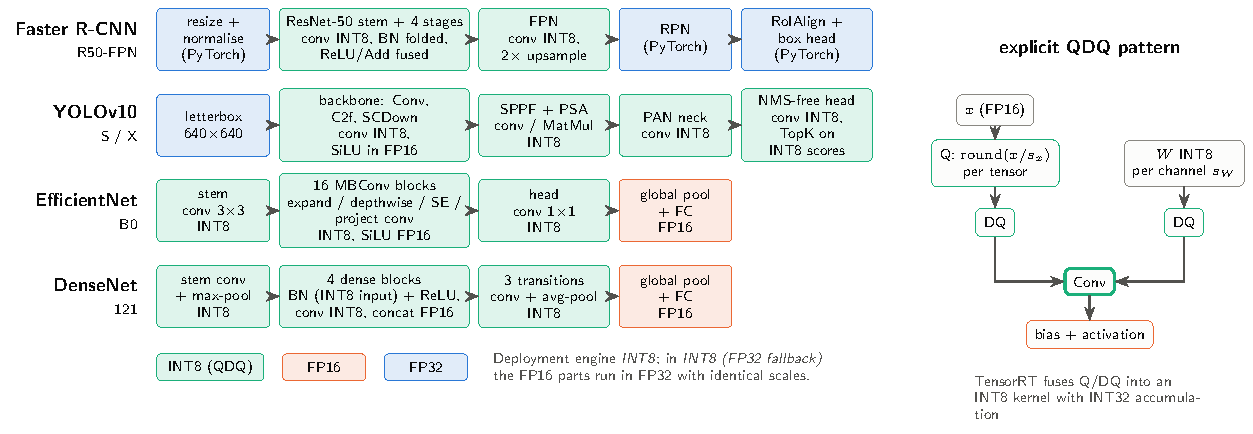
\includegraphics[width=\textwidth]{figures/fig_qdq.pdf}
\caption{Precision of the deployed INT8 engines. Precision of each architectural stage in the deployed INT8 engines (left) and the explicit quantize--dequantize pattern that TensorRT fuses into integer kernels (right). Pre-processing and the Faster R-CNN proposal and ROI heads are not part of the quantized engine.}\label{fig:qdq}
\end{figure}

All variants were compiled with TensorRT~11.3~\cite{tensorrt} into \emph{strongly typed} engines, in which the precision of every layer follows the graph; TF32 was disabled, so that the FP32 baseline is true single precision. Static-shape engines were built for batch sizes 1, 6 and 8, and Faster R-CNN has a dynamic-shape engine (input sides 256--1344) for evaluation; its proposal network and ROI heads run in FP32 PyTorch. The precision in which every convolution is executed was read back from the engine inspector. The environment is listed in Table~\ref{tab:hardware} and implementation details in Supplementary Section~\ref{sec:supp-quant}.

% BEGIN GENERATED M3_hardware
\begin{table}[h]
\caption{Hardware and software environment}\label{tab:hardware}
\begin{tabular}{@{}ll@{}}
\toprule
Component & Version / specification \\
\midrule
GPU & NVIDIA H200, power limit 700 W \\
GPU driver & 590.48.01 \\
CPU & Intel Xeon Platinum 8480C \\
TensorRT & 11.3.0.99 \\
NVIDIA ModelOpt & 0.47.0 \\
ONNX Runtime & 1.24.4 \\
PyTorch / CUDA & 2.11.0+cu128 / 12.8 \\
\botrule
\end{tabular}
\end{table}
% END GENERATED M3_hardware

\subsection{Activation-level deviation metrics}\label{sec:metrics}

Every output tensor of the analysed operators (convolutions, activation functions, additions, pooling, concatenation, resizing and non-foldable batch normalisation) is marked as an engine output, and the strict-FP32 engine is compared with the INT8 (FP32 fallback) engine on identical inputs; marking outputs prevents some fusions but leaves the quantized arithmetic unchanged. With $f$ an FP32 tensor, $q$ its quantized counterpart and $e=q-f$, the metrics of Table~\ref{tab:metrics} are
\begin{align}
\mathrm{MRE}_\mathrm{elem} &= \operatorname*{median}_{i}\frac{|e_i|}{|f_i|+\eta}, \label{eq:mre}\\
A(x,y) &= \max_{c} F(c,x,y), \qquad
\mathrm{MRE}_\mathrm{proj} = \operatorname*{median}_{x,y}\frac{|A_q(x,y)-A_f(x,y)|}{|A_f(x,y)|+\eta}, \label{eq:proj}\\
r &= \frac{\lVert e\rVert_2}{\lVert f\rVert_2}, \qquad \mathrm{SQNR} = 10\log_{10}\frac{\lVert f\rVert_2^2}{\lVert e\rVert_2^2}\ \mathrm{dB}, \label{eq:sqnr}
\end{align}
with $\eta=10^{-6}$. An SQNR of 40, 20 and 0\,dB corresponds to a relative error $r$ of 1\%, 10\% and 100\%; 6\,dB is a factor of two in $r$. Task accuracy is the COCO box mAP@[.5:.95] for detectors~\cite{lin2014microsoft,padilla2021metrics}, complemented for the road-user classes by the AP at IoU 0.5 and by recall and precision at the operating threshold of 0.5, and the top-1 accuracy for classifiers. $\mathrm{MRE}_\mathrm{proj}$ is the metric of the conference paper; $r$ and SQNR are scale-free and standard in the quantization literature~\cite{nagel2021whitepaper}. Per-image values are aggregated over the 500 analysis images by their median and interquartile range. \emph{Head-input} tensors are those consumed by the task head (the five FPN levels, the three YOLOv10 head inputs, the last feature map of the classifiers); for the detectors, $\mathrm{MRE}_\mathrm{proj}$ is also computed inside and outside the ground-truth boxes.

\begin{table}[t]
\caption{PEP-AI metrics. $f$: FP32 tensor, $q$: quantized tensor, $e=q-f$, $A$: channel-wise maximum projection.}\label{tab:metrics}
\begin{tabular}{@{}lllp{4.3cm}@{}}
\toprule
Metric & Definition & PEP-AI role & Interpretation \\
\midrule
$\mathrm{MRE}_\mathrm{proj}$ & Eq.~(\ref{eq:proj}) & precise, explainable & conference-paper metric; spatial, on the dominant response per location \\
$\mathrm{MRE}_\mathrm{elem}$ & Eq.~(\ref{eq:mre}) & precise & element-wise median relative error over all channels \\
$r$ & $\lVert e\rVert_2/\lVert f\rVert_2$ & precise & scale-free relative error; $r\geq1$ means no usable signal \\
SQNR & $-20\log_{10} r$ & precise & signal-to-quantization-noise ratio in dB \\
$a_n$ & $r_\mathrm{out}/\max r_\mathrm{in}$ & explainable & operator-level attenuation ($<1$) or amplification ($>1$) \\
$s_n$ & SQNR drop across node $n$ & explainable & error injected by a layer; drives selective quantization \\
AUC & ROC of deviation vs.\ errors & provable & how well internal deviation predicts detection errors \\
\botrule
\end{tabular}
\end{table}

\subsection{Quantization noise model}\label{sec:noise}

The deviations are interpreted with the additive noise model that underlies analytical range setting~\cite{banner2019aciq,nagel2021whitepaper,gholami2021survey}, under two assumptions. (A1) Inside the clipping range, the INT8 rounding error $e=Q_s(x)-x$ is uniform on $[-s/2,s/2]$ and uncorrelated with $x$, which holds when $s$ is small relative to the spread of $x$. (A2) Under the power-weighted measure $x^2\,\mathrm{d}P(x)$, the significand $m=|x|/2^{\lfloor\log_2|x|\rfloor}$ of an activation is log-uniform on $[1,2)$, which holds approximately for every distribution whose logarithm spreads over several octaves.
\begin{lemma}[Rounding noise]\label{lem:noise}
Let $x$ be an activation with root-mean-square value $\sigma$ and normalised range $\kappa=\alpha/\sigma$. Under (A1), the INT8 quantizer of Eq.~\eqref{eq:int8} with $s=\alpha/127$ has the error power
\begin{equation}
\mathbb{E}\,e^2=\frac{s^2}{12}\Pr\left(|x|\le\alpha\right)+\mathbb{E}\!\left[\left(|x|-\alpha\right)^2\mathbb{1}\{|x|>\alpha\}\right],\label{eq:mse}
\end{equation}
and, without clipping,
\begin{equation}
\mathrm{SQNR}_\mathrm{INT8}=10\log_{10}\!\left(12\cdot127^2\right)-20\log_{10}\kappa\approx52.9\,\mathrm{dB}-20\log_{10}\kappa.\label{eq:sqnr-int8}
\end{equation}
Under (A2), round-to-nearest in a floating-point format with $p$ significand bits has, in its normal range, the error power $\mathbb{E}\,e^2=\mathbb{E}\,x^2\,2^{-2p}/(8\ln2)$, so that, independently of $\kappa$,
\begin{equation}
\mathrm{SQNR}_\mathrm{FP}=20p\log_{10}2+10\log_{10}\left(8\ln2\right)\approx6.02\,p+7.44\,\mathrm{dB}.\label{eq:sqnr-fp}
\end{equation}
\end{lemma}
For E4M3 ($p=4$) Eq.~\eqref{eq:sqnr-fp} gives 31.5\,dB and for FP16 ($p=11$) 73.7\,dB: the relative precision of a floating-point format does not depend on the calibrated range~\cite{kuzmin2022fp8,vanbaalen2023fp8}, whereas INT8 loses 20\,dB per decade of $\kappa$, and Eq.~\eqref{eq:mse} formalises the trade-off between the granular noise of a wide range and the clipping of a narrow one~\cite{banner2019aciq,zhao2019ocs}. A Monte Carlo simulation reproduces Eqs.~\eqref{eq:mse}--\eqref{eq:sqnr-fp} within 0.1\,dB (Fig.~\ref{fig:noise}); the proofs are given in Supplementary Section~\ref{sec:supp-noise}. Because TensorRT uses static scales, Lemma~\ref{lem:noise} also predicts the effect of a change of the signal level after calibration.
\begin{corollary}[Static scales]\label{cor:static}
Let the scale $s$ be calibrated for an activation with root-mean-square value $\sigma_\mathrm{cal}$, and let the activation at inference be $c$ times larger in distribution, $c>0$. If no value is clipped and (A1), (A2) hold, then
\begin{equation}
\Delta\mathrm{SQNR}_\mathrm{INT8}=20\log_{10}c,\qquad\Delta\mathrm{SQNR}_\mathrm{FP8}=0\quad\text{for }c\,\sigma_\mathrm{cal}\gg2^{-6}s,\label{eq:static}
\end{equation}
where $2^{-6}s$ is the smallest normal E4M3 number.
\end{corollary}
INT8 loses 6\,dB per halving of the signal, FP8 nothing, and a signal that grows ($c>1$) enters the clipping regime of Eq.~\eqref{eq:mse}, which the tight INT8 range, unlike the maximum-calibrated FP8 range, cannot absorb. Reduced contrast and fog are such shifts; the attenuation $c$ has to be measured at the quantizers, because biases and mean responses do not scale with the pixel contrast (Supplementary Section~\ref{sec:supp-noise}).

\pepfigure{M_noise_model}{Quantization noise model (lines: Eqs.~\eqref{eq:mse}--\eqref{eq:sqnr-fp}; markers: Monte Carlo simulation with $4\times10^5$ samples). \textbf{a} SQNR of INT8 versus the normalised clipping range $\kappa=\alpha/\sigma$ for Gaussian and Laplacian signals, and of FP8 E4M3. \textbf{b} SQNR of a signal attenuated by the factor $c$ after the scale was calibrated at $\kappa_\mathrm{cal}=8$ (static per-tensor scale); vertical lines: contrast factors of the five COCO-C contrast severities.}{fig:noise}

\subsection{Error propagation model}\label{sec:propagation}

The conference paper modelled the propagation of quantization error between layers $l$ and $l+1$ as
\begin{equation}
\epsilon^{(l+1)} = \mathcal{A}\left(\mathcal{F}(y_f^{(l)}+\epsilon^{(l)})-\mathcal{F}(y_f^{(l)})\right)+\delta^{(l+1)},
\label{eq:attenuation}
\end{equation}
with layer transformation $\mathcal{F}$, local rounding noise $\delta^{(l+1)}$ and an attenuation operator $\mathcal{A}$; analytical treatments propagate quantization noise under distributional assumptions~\cite{sakr2017analytical} or constrain layers to be non-expansive~\cite{lin2019defensive}. Here every node $n$ is linearised around its FP32 operating point. With FP32 output $x_n$, deviation $e_n$, inputs $\pi(n)$, Jacobian $J_n$ and injected rounding noise $\delta_n$ ($\delta_n=0$ without quantizers),
\begin{equation}
e_n=J_n\,e_{\pi(n)}+\delta_n,\label{eq:linear}
\end{equation}
where $e_{\pi(n)}$ stacks the deviations of all inputs. Squared norms of deviations are understood as expectations over the rounding noise, $\lVert e\rVert^2:=\mathbb{E}\,\lVert e\rVert^2$. For $\delta_n$ uncorrelated with the propagated deviation, the cross term $2\,\mathbb{E}\langle J_ne_{\pi(n)},\delta_n\rangle$ vanishes, and the relative error $r_n=\lVert e_n\rVert/\lVert x_n\rVert$ obeys
\begin{equation}
r_n^2=g_n^2\,r_{\pi(n)}^2+\rho_n^2,\qquad g_n=\frac{\lVert J_n e_{\pi(n)}\rVert}{\lVert e_{\pi(n)}\rVert}\cdot\frac{\lVert x_{\pi(n)}\rVert}{\lVert x_n\rVert},\qquad\rho_n=\frac{\lVert\delta_n\rVert}{\lVert x_n\rVert}.\label{eq:recursion}
\end{equation}
The propagation gain $g_n$ is the attenuation operator $\mathcal{A}$ in scalar form. For every analysed node we measure the amplification ratio
\begin{equation}
a_n=\frac{r_n}{\max_{m\in\pi(n)}r_m}\leq\sqrt{g_n^2+\rho_n^2/r_{\pi(n)}^2},\label{eq:amplification}
\end{equation}
with equality for single-input nodes, because $r_{\pi(n)}\leq\max_m r_m$ for stacked inputs; for single-input operators without quantizers $a_n=g_n$. Closed forms of $g_n$ for sigmoid gates, max pooling and non-folded batch normalisation (Eq.~\eqref{eq:bn}) are derived in Supplementary Section~\ref{sec:supp-prop}, where the following two statements are also proved.
\begin{proposition}\label{prop:selective}
Assume the linearisation of Eq.~\eqref{eq:linear} and zero-mean, mutually uncorrelated injected noises $\delta_n$. Then the relative error at the head input $h$ is
\begin{equation}
r_h^2=\sum_{n}\Gamma_{n\to h}\,\rho_n^2,\qquad\Gamma_{n\to h}=\frac{\mathbb{E}\lVert J_{n\to h}\,\delta_n\rVert^2}{\mathbb{E}\lVert\delta_n\rVert^2}\cdot\frac{\lVert x_n\rVert^2}{\lVert x_h\rVert^2},\label{eq:additive}
\end{equation}
where $J_{n\to h}$ is the Jacobian from node $n$ to $h$. Keeping a set $S$ of nodes in FP16, whose injected noise is negligible by Eq.~\eqref{eq:sqnr-fp}, gives $r_h^2(S)=r_h^2-\sum_{n\in S}\Gamma_{n\to h}\,\rho_n^2$, and a set of $k$ nodes that minimises $r_h^2(S)$ consists of the $k$ largest contributions $\Gamma_{n\to h}\,\rho_n^2$.
\end{proposition}
\begin{proposition}\label{prop:fixedpoint}
Let a chain of nodes $1,\dots,n$ satisfy Eq.~\eqref{eq:recursion} with gains $g_m$ and injected noise $\rho_m$. Then
\begin{equation}
r_n^2=r_0^2\prod_{m=1}^{n}g_m^2+\sum_{k=1}^{n}\rho_k^2\prod_{m=k+1}^{n}g_m^2.\label{eq:unrolled}
\end{equation}
If $g_m\le\bar g<1$ and $\rho_m\le\bar\rho$ for all $m$, the relative error stays bounded by $\max\{r_0,\ \bar\rho/\sqrt{1-\bar g^2}\}$ at any depth, and for constant $g_m=g<1$ and $\rho_m=\rho$ it converges to the fixed point
\begin{equation}
r_\infty=\frac{\rho}{\sqrt{1-g^2}},\qquad \mathrm{SQNR}_\infty=-20\log_{10}\rho+10\log_{10}\left(1-g^2\right).\label{eq:fixedpoint}
\end{equation}
If instead $g_m\ge g>1$, the propagated part grows at least as $g^{2n}r_0^2$.
\end{proposition}
Proposition~\ref{prop:fixedpoint} formalises the attenuation effect of the conference paper: the error need not shrink from layer to layer; a contraction of its propagated part ($g<1$) suffices for a plateau $r_\infty$ determined by $\rho$ and $g$. Proposition~\ref{prop:selective} motivates selective precision and a prediction of the head-input fidelity from FP32 statistics alone: applying Eq.~\eqref{eq:int8} with the calibrated scales to FP32 activations gives the injected noise $\rho_n^2$ of every quantizer exactly, and unit propagation factors give
\begin{equation}
\mathrm{SQNR}_\mathrm{add}=-10\log_{10}\sum_n\rho_n^2,\qquad\bar\Gamma=\frac{r_h^2}{\sum_n\rho_n^2}=10^{(\mathrm{SQNR}_\mathrm{add}-\mathrm{SQNR}_h)/10},\label{eq:gammabar}
\end{equation}
where $\mathrm{SQNR}_h$ is the measured head-input SQNR. By Proposition~\ref{prop:selective}, $\bar\Gamma=\sum_n\Gamma_{n\to h}\rho_n^2/\sum_n\rho_n^2$ is the mean propagation factor weighted by the injected noise; it is below one for networks that attenuate the injected noise and above one for networks that amplify it (Fig.~\ref{fig:propmodel}).

\begin{figure}[t]
\centering
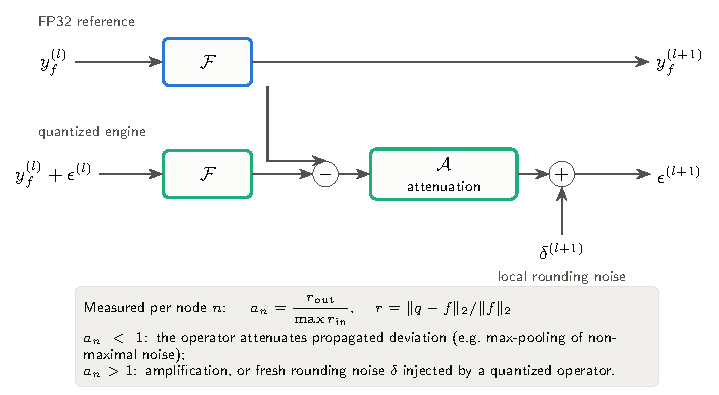
\includegraphics[width=0.85\textwidth]{figures/fig_propagation_model.pdf}
\caption{Error propagation model. Model of the conference paper (Eq.~\ref{eq:attenuation}) and the per-node amplification ratio used to estimate the attenuation operator $\mathcal{A}$ from measured activations.}\label{fig:propmodel}
\end{figure}

\subsection{Deviation--risk analysis}\label{sec:risk}

Both engines are run on all 5\,000 validation images with the head-input tensors exposed and compared at a score threshold of 0.5. As in the conference paper, an image contains a \emph{detection error} if a ground-truth object found by FP32 is missed by INT8 or if an FP32 detection has no same-class INT8 counterpart with IoU $\geq0.5$; a \emph{score-tolerant} variant accepts INT8 counterparts down to a score of 0.3, so that an FP32 detection without a counterpart has genuinely vanished. The image-level ROC AUC of the head-input $\mathrm{MRE}_\mathrm{proj}$ is compared with that of a trivial covariate, the number of FP32 detections, and an architecture-specific threshold of the local deviation defined below is derived from the data as the cut that maximises Youden's index $J=\mathrm{TPR}-\mathrm{FPR}$ for vanishing detections. At the detection level, the \emph{local deviation} $d_j$ of detection $j$, the median $\mathrm{MRE}_\mathrm{proj}$ of the head-input maps inside its box, enters the logistic model
\begin{equation}
\operatorname{logit}\Pr(v_j=1)=\beta_0+\beta_1\log_2 d_j+\beta_2\,m_j+\beta_3\log A_j\label{eq:logit}
\end{equation}
for its vanishing $v_j$, with score margin $m_j=-|s_j-0.5|$ and box area $A_j$; $e^{\beta_1}$ is the odds ratio per doubling of the local deviation. These analyses use the INT8 engines with FP32 fallback. The consequence of box shifts for monocular distance estimation follows from a flat-ground camera model (Supplementary Section~\ref{sec:supp-risk}).

\subsection{Latency, jitter and energy}\label{sec:energy}

Latency was measured on the otherwise idle GPU, one engine at a time, with CUDA events around each of 2\,000 executions after 100 warm-up runs, with and without CUDA graphs, on device-resident inputs; pre-processing, host transfers and the Faster R-CNN detection heads are excluded, so that the measurement isolates the compiled engine. Latencies are summarised by the median (p50), the 99th percentile (p99), the maximum and the jitter $Q_{0.99}-Q_{0.5}$. Energy was read from the GPU energy counter $E(t)$ (NVML) during at least 20\,s of sustained execution of $n$ batches of size $B$, replayed as CUDA graphs like the latency measurements, after 10\,s of idling at power $P_\mathrm{idle}$:
\begin{equation}
E_\mathrm{img}=\frac{E(t_1)-E(t_0)}{nB},\qquad E_\mathrm{img}^\mathrm{net}=E_\mathrm{img}-\frac{P_\mathrm{idle}\,(t_1-t_0)}{nB}.\label{eq:energy}
\end{equation}
Sustained runs average out the partial sampling of the built-in power sensor~\cite{yang2024gpuenergy}; clock and temperature were logged, and every measurement was repeated three times (median). Memory traffic and the executed precision of every layer were read from the engine inspector (Eq.~\eqref{eq:traffic}); reference energies per operation~\cite{horowitz2014energy} are given in Table~\ref{tab:energyref}.

% BEGIN GENERATED M5_energy_reference
\begin{table}[h]
\caption{Energy per operation at 45\,nm (Horowitz, ISSCC 2014)}\label{tab:energyref}
\begin{tabular}{@{}lr@{}}
\toprule
Operation & Energy (pJ) \\
\midrule
8-bit integer add & 0.03 \\
32-bit integer add & 0.1 \\
16-bit float add & 0.4 \\
32-bit float add & 0.9 \\
8-bit integer multiply & 0.2 \\
32-bit integer multiply & 3.1 \\
16-bit float multiply & 1.1 \\
32-bit float multiply & 3.7 \\
32-bit SRAM read (8 kB) & 5 \\
32-bit DRAM read & 640 \\
\botrule
\end{tabular}
\end{table}
% END GENERATED M5_energy_reference

\subsection{Robustness under adverse imaging conditions}\label{sec:robustness}

Fog, snow, frost, brightness (glare), contrast, Gaussian sensor noise and motion blur follow the COCO-C protocol~\cite{michaelis2019benchmarking,hendrycks2019benchmarking} at severities 1--5 with fixed per-image seeds; low light is simulated by gamma darkening with Poisson shot noise (Fig.~\ref{fig:conditions}). For every condition, severity and precision, box mAP, head-input deviation and detection-error rate are reported on the 500 analysis images. Two label-free remedies were tested for the YOLOv10 detectors: a robust calibration set in which half of the images carry a random condition, and keeping the input or the top-ranked convolution in FP16.

\pepfigure{M_conditions}{Adverse imaging conditions. The eight adverse imaging conditions applied to a COCO val2017 traffic scene (image 336232) at severity 3 of 5. Low light is gamma darkening with Poisson shot noise; the other conditions follow the COCO-C protocol.}{fig:conditions}

\subsection{PEP-AI-guided diagnosis and repair}\label{sec:selective}

The main INT8 results use the default placement and entropy calibration of the toolchain. Every model is additionally re-quantized in a configuration chosen exclusively with label-free criteria on the calibration split, namely the head-input SQNR and the output consistency with FP32 (Eq.~\eqref{eq:consistency}): (i) the calibration method, (ii) the placement of operators whose measured amplification shows that they magnify upstream noise, such as the pre-activation batch normalisation of DenseNet, and (iii) selective precision. For selective precision, the sensitivity of a convolution is the median SQNR drop across it, $s_n=20\log_{10}a_n$ (for the input convolution $\max(0,40\,\mathrm{dB}-\mathrm{SQNR}_n)$); the $k$ most sensitive convolutions are kept in FP16 (one-shot), or the network is re-measured after every exclusion (iterative; Algorithm~\ref{alg:selective}). All variants share the calibration scales of the base model (Supplementary Section~\ref{sec:supp-repair}). Unlike Hessian-based allocation~\cite{dong2019hawq,yao2021hawqv3} or reconstruction-based PTQ~\cite{li2021brecq,wei2022qdrop}, no gradients are needed. The ranking is compared with random subsets (three seeds), the all-depthwise heuristic~\cite{sheng2018quantization,nagel2019datafree} and a ranking predicted from FP32 statistics alone. Task accuracy is measured only afterwards.

\subsection{AI-based business optimisation (AIBO) scenario}\label{sec:aibo}

The measured energy per image at batch size 6, i.e.\ the synchronised frames of the six cameras of a vehicle, is scaled to a fleet of $N=\text{vehicles}\times\text{cameras}\times\text{frame rate}\times\text{operating hours}$ inferences per year, with the EU non-household electricity price of 0.1837\,EUR/kWh (second half of 2025)~\cite{eurostat2026prices} and the EU grid intensity of 242\,g\,CO$_2$/kWh (2023)~\cite{ember2024eer} as reference values, bracketed by 0.10--0.30\,EUR/kWh and 100--400\,g/kWh. Following the AIBO view of AI as an input to managerial decisions~\cite{duan2019decision}, the annual cost of a precision $p$ is
\begin{equation}
C(p,\lambda) = N\,E_\mathrm{img}(p)\,c_\mathrm{el} + N\,K(p)\,\lambda,\label{eq:aibo}
\end{equation}
with electricity price $c_\mathrm{el}$, penalty $\lambda$ per critical error and $K(p)$ critical errors per image relative to FP32: FP32 detections of road users (person, bicycle, car, motorcycle, bus, truck) that vanish in the deployed engine under the score-tolerant definition, or top-1 disagreements for classifiers. Because $K(\mathrm{FP32})=0$, the \emph{break-even penalty}
\begin{equation}
\lambda^*(p) = \frac{\left(E_\mathrm{img}(\mathrm{FP32})-E_\mathrm{img}(p)\right)c_\mathrm{el}}{K(p)}\label{eq:breakeven}
\end{equation}
is the cost per critical error above which the saving of $p$ no longer pays off, and the lower envelope of $C(\cdot,\lambda)$ gives the cost-optimal precision for every $\lambda$ (Fig.~\ref{fig:aibo}). Only the GPU inference energy is counted (no host, cooling or idle power), and false positives, such as duplicate boxes, are not counted as critical errors. The absolute figures describe a fleet whose onboard accelerator has the measured energy per image of the H200; for an embedded GPU they scale with its own energy per image, whereas the relative savings and the structure of Eqs.~\eqref{eq:aibo}--\eqref{eq:breakeven} carry over.

\begin{figure}[t]
\centering
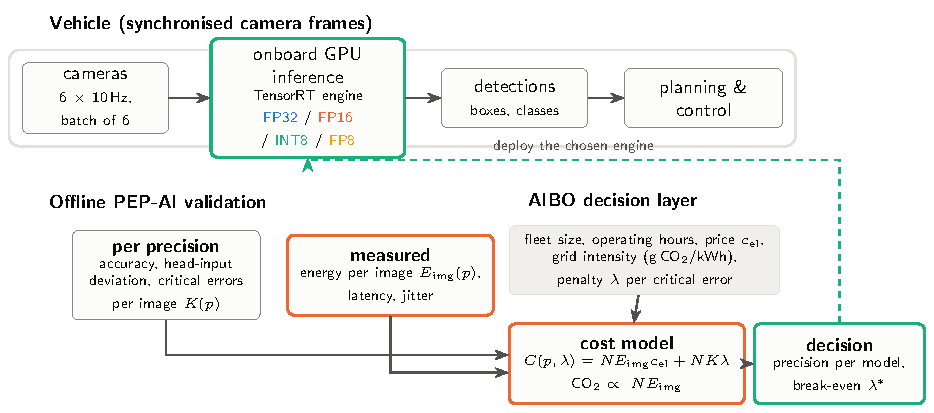
\includegraphics[width=0.95\textwidth]{figures/fig_aibo.pdf}
\caption{AIBO view of quantized perception. Offline PEP-AI validation supplies accuracy, deviation, the critical errors per image $K(p)$ and the measured energy per image $E_\mathrm{img}(p)$ of every precision; combined with fleet parameters, electricity price, grid intensity and a penalty $\lambda$ per critical error, the cost model of Eq.~\eqref{eq:aibo} selects the precision of each deployed engine.}\label{fig:aibo}
\end{figure}

\subsection{Statistical analysis}\label{sec:stats}

Accuracy differences to FP32 carry 95\% confidence intervals from 1\,000 paired bootstrap resamples of the evaluation images (Eq.~\eqref{eq:bootstrap}); the discriminative power of a deviation score is the ROC AUC, the Mann--Whitney probability that an erroneous case scores higher than a correct one, with bootstrap intervals, and odds ratios carry bootstrap intervals over detections. Medians are reported with interquartile ranges where the spread across images is of interest. All random choices are seeded.

\subsection{Static analysis of the FP32 parameters}\label{sec:static}
The first steps of the procedure in Section~\ref{sec:worked} need calibration images. A coarser version needs none: the weights and the batch-normalisation (BN) buffers of the FP32 model already determine most quantities, without an image and without a forward pass (\texttt{43\_static\_analysis.py}). The analysis is static by design; executing the model on an image folder (\texttt{44\_validate\_static.py}) serves only to validate it (Section~\ref{sec:res-static}).

\emph{Weights.} For every convolution and linear layer, with BN folded as in deployment, the weights $w_c$ of output channel $c$ are quantized exactly with $s_c=\max|w_c|/127$ (INT8, per channel), with one scale for the whole tensor, and to E4M3 with $s_c=\max|w_c|/448$; the SQNR is computed from the quantized and original weights, without approximation. By Lemma~\ref{lem:noise} it is about $52.9\,\mathrm{dB}-20\log_{10}\kappa_w$ with $\kappa_w=\max|w_c|/\mathrm{RMS}(w_c)$: outlier weights lower it, the number of weights does not.

\emph{Activations.} A BN layer stores the running mean $\mu_c$ and variance $v_c$ of its input, so that its output channel $c$ has mean $\beta_c$ and standard deviation $\sigma_c=|\gamma_c|\sqrt{v_c/(v_c+\epsilon)}$. Each channel is modelled as Gaussian, $N(\beta_c,\sigma_c^2)$, passed through the following activation function: a ReLU turns it into a rectified Gaussian with a point mass at zero, which uses only the positive half of the symmetric INT8 grid, and SiLU leaves a small negative tail bounded by $-0.28$. The tensor is the mixture of its channels; with channels of different width this mixture is heavy-tailed, so that the per-tensor range $\alpha$ is set by the widest channels while the narrow ones are quantized coarsely. The range is chosen to minimise the error power of Eq.~\eqref{eq:mse} on this mixture (2\,048 synthetic samples per channel), which gives $\kappa=\alpha/\sigma$ and the injected SQNR of Lemma~\ref{lem:noise}; FP8 uses the maximum. The channel imbalance is reported as the ratio of the 90th to the 10th percentile of the channel RMS. Summing the injected noise of all $N$ modelled tensors and, optionally, of the weights gives a static $\mathrm{SQNR}_\text{add}$ by Eq.~\eqref{eq:gammabar}, and the gain of every BN that cannot be folded follows from Eq.~\eqref{eq:bn}.

\emph{How the network enters.} The static $\mathrm{SQNR}_\text{add}=-10\log_{10}N-10\log_{10}\langle\rho_n^2\rangle$ falls by 3\,dB per doubling of the number of quantized tensors, i.e.\ with depth. Width enters only through the channel imbalance, spatial size and parameter count not at all. Because $\langle\rho_n^2\rangle$ is a mean of noise powers, it is dominated by the weakest tensors: those with a large $\kappa$ from outlier channels, depthwise inputs, gates or attention blocks. Through the propagation factor and the relation of Section~\ref{sec:worked}, a lower head-input SQNR translates into a relative accuracy loss that grows roughly tenfold per 12\,dB. What the static analysis cannot see is the propagation factor itself, tensors without a BN (such as the outputs of residual additions), heavier-than-Gaussian tails of real activations and errors created by decoders and heads.

\emph{Example.} In MobileNetV2, not used elsewhere in this article, the BN after the projection convolution of block~6 (\texttt{features.6.conv.3}, no activation) has $C=32$ channels with $\beta_c\approx0$ and $\sigma_c$ between 1.04 and 12.36, a tensor RMS of 3.60 and a channel imbalance of 3.8. The MSE-optimal range is $\alpha=40.9$, i.e.\ $\kappa=11.36$, and Eq.~\eqref{eq:sqnr-int8} gives $52.87-20\log_{10}11.36=52.87-21.11=31.8$\,dB, against 31.2\,dB from the quantized samples (no clipping). The step $s=\alpha/127=0.32$ is 0.03 of the widest channel but 0.31 of the narrowest, whose own SQNR is only $10\log_{10}\bigl(12\,\sigma_c^2/s^2\bigr)=10\log_{10}(12/0.31^2)=20.9$\,dB, against 42.5\,dB for the widest: a per-tensor scale makes the narrow channels about 22\,dB noisier. Over the network, the 52 modelled tensors have a mean injected noise of 39.1\,dB, so that $\mathrm{SQNR}_\text{add}=39.1-10\log_{10}52=39.1-17.2=22.0$\,dB without and 20.3\,dB with the 53 weight layers; FP8 gives 12.0\,dB, because E4M3 weights (about 32\,dB) contribute as much noise as its activations.

\section{Results}\label{sec:results}

\subsection{Deployment efficiency on the GPU}\label{sec:res-speed}
INT8 is the fastest deployment format for Faster R-CNN, YOLOv10-X and EfficientNet-B0 at both batch sizes and for YOLOv10-S at batch size 8, where it is within 1\% of FP8 at batch size 1 (Fig.~\ref{fig:speed}, Table~\ref{tab:accuracy}). Relative to strict FP32 it lowers the median latency 1.6--8.5-fold at batch size 1 and 2.3--11.8-fold at batch size 8 (Faster R-CNN: 40.7 to 3.5\,ms per batch), and it is 1.12--1.27 and 1.24--1.47 times faster than FP16, so its advantage does not rest on the FP32 baseline alone. At batch size 8, INT8 needs 72--91\% less energy per image than FP32 and 37--49\% less than FP16 (Faster R-CNN 281 instead of 3\,184\,mJ, YOLOv10-X 295 instead of 2\,477\,mJ; 80--91\% less above idle), and its weights occupy 25--32\% of their FP32 size. With CUDA graphs, latency is highly deterministic: the jitter is at most 0.015\,ms for every INT8 engine and 0.08\,ms for any engine, and the slowest of 2\,000 executions exceeds the median by at most 23\% (EfficientNet-B0 in FP8, 0.64 versus 0.52\,ms), which bounds the observed worst-case execution time. The three repeats of each measurement differ by a median of 0.1\% in latency and 0.5\% in energy (at most 8.8\% and 6.0\%), well below the differences between formats. The engine inspector attributes the gains to the number format (Table~\ref{tab:engines}): every quantized convolution runs on INT8 kernels, and INT8 cuts the memory traffic per inference to 14--26\% of FP32 (FP16: 40--62\%, FP8: 26--39\%). FP8 is slower than INT8 wherever its activation functions run as separate kernels, which doubles the activation traffic of YOLOv10-X, but faster for DenseNet-121 (1.23 versus 1.85\,ms at batch size 8), whose concatenations the conventional engines implement as hundreds of copies. Power-limit throttling, launch overhead and output conversion costs are detailed in Supplementary Section~\ref{sec:supp-res-speed}.

\pepfigure{R5_speedup}{Deployment efficiency on the NVIDIA H200 (TensorRT~11.3, CUDA graphs). \textbf{a, b} Speed-up of the median latency over strict FP32 at batch sizes 1 and 8. \textbf{c} Deployed weight size. \textbf{d} Gross GPU energy per image at batch size 8 (NVML, sustained CUDA-graph execution; logarithmic axis).}{fig:speed}

% BEGIN GENERATED R1_accuracy_speed
\begin{sidewaystable}
\footnotesize\setlength{\tabcolsep}{4pt}
\caption{Task accuracy, latency, throughput and energy per precision (TensorRT 11.3, NVIDIA H200)}\label{tab:accuracy}
\begin{tabular}{@{}llrlrrrr@{}}
\toprule
Model & Precision & Accuracy (\%) & $\Delta$ vs FP32 [95\% CI] & p50 bs1 (ms) & p99 bs1 (ms) & Images/s bs8 & mJ/image bs8 \\
\midrule
Faster R-CNN R50-FPN & FP32 & 37.0 & -- & 6.29 & 6.32 & 197 & 3184 \\
 & FP16 & 36.9 & $-$0.01 [$-$0.04, $+$0.02] & 0.91 & 0.92 & 1571 & 443 \\
 & INT8 & 36.7 & $-$0.25 [$-$0.36, $-$0.13] & 0.74 & 0.74 & 2312 & 281 \\
 & FP8 & 36.6 & $-$0.37 [$-$0.49, $-$0.25] & 0.91 & 0.92 & 1770 & 392 \\
\midrule
YOLOv10-S & FP32 & 46.0 & -- & 1.78 & 1.78 & 1269 & 409 \\
 & FP16 & 46.0 & $+$0.01 [$-$0.03, $+$0.03] & 0.81 & 0.81 & 4370 & 109 \\
 & INT8 & 43.8 & $-$2.24 [$-$2.56, $-$1.83] & 0.69 & 0.69 & 5430 & 63.3 \\
 & FP8 & 45.6 & $-$0.41 [$-$0.53, $-$0.28] & 0.68 & 0.69 & 4297 & 96.7 \\
\midrule
YOLOv10-X & FP32 & 54.0 & -- & 6.06 & 6.07 & 239 & 2477 \\
 & FP16 & 54.0 & $-$0.01 [$-$0.07, $+$0.02] & 1.99 & 2.00 & 1160 & 582 \\
 & INT8 & 47.8 & $-$6.21 [$-$6.52, $-$5.74] & 1.57 & 1.57 & 1658 & 295 \\
 & FP8 & 53.9 & $-$0.15 [$-$0.31, $-$0.01] & 1.79 & 1.79 & 1375 & 430 \\
\midrule
EfficientNet-B0 & FP32 & 65.8 & -- & 0.59 & 0.60 & 7086 & 45.7 \\
 & FP16 & 65.8 & $-$0.02 [$-$0.12, $+$0.06] & 0.42 & 0.42 & 12087 & 20.6 \\
 & INT8 & 24.8 & $-$40.97 [$-$42.07, $-$39.77] & 0.38 & 0.38 & 16564 & 12.7 \\
 & FP8 & 65.4 & $-$0.39 [$-$0.79, 0.00] & 0.52 & 0.52 & 9598 & 26.0 \\
\midrule
DenseNet-121 & FP32 & 62.0 & -- & 2.78 & 2.79 & 1912 & 152 \\
 & FP16 & 62.0 & $-$0.02 [$-$0.11, $+$0.07] & 1.59 & 1.59 & 3344 & 70.5 \\
 & INT8 & 57.4 & $-$4.68 [$-$5.37, $-$3.98] & 1.39 & 1.39 & 4325 & 40.6 \\
 & FP8 & 61.7 & $-$0.32 [$-$0.64, $+$0.02] & 0.71 & 0.71 & 6510 & 40.9 \\
\botrule
\end{tabular}
\footnotetext{Accuracy: COCO val2017 box mAP@[.5:.95] (5\,000 images) for detectors, ImageNetV2 top-1 (9\,000 images) for classifiers; 95\% CI of the difference from 1\,000 paired bootstrap resamples of the images. Latency: median (p50) and 99th percentile (p99) of 2\,000 executions with CUDA graphs; throughput from the mean latency with CUDA graphs. Energy: gross GPU energy per image from the NVML counter during sustained CUDA-graph execution. Median of three repeats. INT8 and FP8 engines keep non-quantized operations in FP16; INT8 uses the entropy calibration of the toolchain on the full calibration set in its stored order (sensitivity: Table~\ref{tab:calibvar}); Faster R-CNN: backbone and FPN only.}
\end{sidewaystable}
% END GENERATED R1_accuracy_speed

\subsection{Task accuracy of the quantized engines}\label{sec:res-accuracy}

The FP32 engines reproduce the published accuracies (Faster R-CNN 36.95 mAP versus 37.0, YOLOv10-S 46.0 versus 46.3, YOLOv10-X 54.0 versus 54.4). These are competitive values: COCO mAP averages the precision over 80 classes and ten IoU thresholds up to 0.95~\cite{lin2014microsoft,padilla2021metrics}, current real-time detectors reach 51--55~\cite{wang2023yolov7,zhao2024rtdetr,wang2024yolov10}, and for road users the FP32 detectors reach an AP$_{50}$ of 82--86\% for persons and 68--76\% for cars and find 88--93\% of the large ones at the operating threshold (Table~\ref{tab:operating}). The ImageNetV2 accuracies of the classifiers, 65.8\% and 62.0\%, correspond to 77.7\% and 74.4\% on the original ImageNet validation set~\cite{torchvision2016}, the known shift of ImageNetV2~\cite{recht2019imagenet,taori2020measuring}. FP16 matches FP32 within 0.02 points, with paired 95\% confidence intervals that include zero (Table~\ref{tab:accuracy}). Every INT8 loss is significant and depends on the architecture: Faster R-CNN loses 0.25 mAP (CI 0.13--0.36), YOLOv10-S and YOLOv10-X 2.2 and 6.2 mAP, DenseNet-121 4.7 top-1 points, and EfficientNet-B0 collapses from 65.8\% to 24.8\%. FP8 loses at most 0.4 points, as Eq.~\eqref{eq:sqnr-fp} predicts for a format whose relative precision does not depend on the range; only for Faster R-CNN, whose INT8 quantizers operate at moderate ranges ($\kappa\approx18$), is it marginally worse than INT8 (36.58 versus 36.71). The head-input SQNR follows the accuracy (15.0, 13.4 and 16.7\,dB for FP8 against 11.6, $-0.9$ and 6.6\,dB for INT8 in YOLOv10-S, EfficientNet-B0 and DenseNet-121).

The YOLOv10 losses concentrate on large objects (mAP$_\text{large}$ $-7.7$ and $-13.2$), although their localisation is unchanged (best IoU 0.947 versus 0.950 for YOLOv10-X). For YOLOv10-X the cause is structural: its NMS-free one-to-one head suppresses duplicates implicitly~\cite{wang2024yolov10}, and INT8 breaks this suppression, so that 15.2\% of its detections above the operating threshold duplicate a higher-scoring box of the same class (IoU $\geq0.7$), against 0.25\% for FP32 and FP8 (Table~\ref{tab:duplicates}). Class-wise non-maximum suppression, which leaves FP32 and FP8 unchanged, raises the INT8 mAP from 47.8 to 52.4 and mAP$_\text{large}$ from 57.2 to 65.7 for 0.16\,ms per image (10\% of the engine latency at batch size 1); the remainder coincides with lower class scores of large objects (median 0.92 in FP32, 0.85 in INT8). YOLOv10-S shows no such effect (0.55\% duplicates); its default quantizer placement had cost it another 0.9 mAP through the quantized TopK and box decoder, a deployment artefact that output-level metrics would have attributed to the network (Supplementary Section~\ref{sec:supp-quant}).

The INT8 accuracy of the fragile networks also depends on the range setting (Tables~\ref{tab:calibmethods} and~\ref{tab:calibvar}). The toolchain builds its entropy histogram one image at a time, so that the first calibration image fixes a lower bound of every clipping range (Supplementary Section~\ref{sec:supp-quant}). Calibration subsets that begin with other images leave Faster R-CNN, the network with the smallest propagation factor, unchanged ($\pm0.01$ mAP), but move YOLOv10-X by up to 2.7 mAP and EfficientNet-B0 from 24.8\% to 41.7\%. An order-independent entropy calibration raises DenseNet-121 to 60.0\% but over-clips the SiLU networks (YOLOv10-X 37.1 mAP). No INT8 range setting is best for all networks, whereas FP8, whose precision does not depend on the range (Lemma~\ref{lem:noise}), stays within 0.4 points of FP32 for all of them (Supplementary Section~\ref{sec:supp-res-calib}).

\subsection{Activation-level deviation}\label{sec:res-activations}
The FP16 engines deviate from FP32 by a head-input SQNR of 36.9--50.5\,dB, the numerical floor of the comparison. The INT8 deviations are one to two orders of magnitude larger and ordered like the accuracy losses (Table~\ref{tab:layerstats}): the head-input $\mathrm{MRE}_\mathrm{proj}$ is 2.0\% for Faster R-CNN, 5.8\% for YOLOv10-S, 13.4\% for DenseNet-121, 14.4\% for YOLOv10-X and 25.9\% for EfficientNet-B0. Within the ground-truth object regions the relative deviation is lower than in the background for every detector (Faster R-CNN 2.9\% vs.\ 3.3\%, YOLOv10-S 3.9\% vs.\ 6.2\%, YOLOv10-X 6.4\% vs.\ 13.2\%; Fig.~\ref{fig:maps}), as the additive model predicts, because the same absolute noise is smaller relative to the stronger object responses (Eq.~\eqref{eq:spatial}). The hexbin densities (Fig.~\ref{fig:hexbin}) show why fragile networks fail: for EfficientNet-B0 a diagonal of deviations equal to minus the FP32 value marks activations rounded to zero by a too coarse per-tensor scale.

Along the depth (Fig.~\ref{fig:propagation}) the SQNR falls within the first layers and then stabilises, as Proposition~\ref{prop:fixedpoint} predicts: the chain recursion fitted to consecutive convolutions gives $g=0.90$, 0.60 and 0.70 ($R^2=0.68$, 0.13 and 0.24, because branches break the chain order) and fixed points of 18.5, 13.7 and 5.7\,dB against measured plateaus of 20.3, 13.5 and 6.0\,dB for Faster R-CNN, YOLOv10-S and YOLOv10-X; the densely branched EfficientNet-B0 and DenseNet-121 do not form chains and require the graph form of Proposition~\ref{prop:selective}. FP8 lies between INT8 and FP16 along the whole depth (median layer SQNR 14.3--21.5\,dB against 5.0--19.8\,dB for INT8). The operator ratios (Fig.~\ref{fig:operators}) quantify the attenuation of the conference paper per operator type: sigmoid gates attenuate ($a_n=0.30$--0.54), max pooling only where no quantizer precedes it, and non-folded batch normalisation amplifies (median 1.17 per layer in DenseNet), as its closed form predicts from the FP32 parameters alone (Eq.~\eqref{eq:bn}: median 1.24; Spearman $\rho=0.83$ over 62 layers).

The additive model connects these observations with the network-level fidelity (Table~\ref{tab:propagation}, Fig.~\ref{fig:noisevalidation}). Every INT8 quantizer is benign on its own (median injected SQNR 26.7--32.5\,dB, predicted within 1.1--2.8\,dB by Eq.~\eqref{eq:sqnr-int8}). Summed with unit propagation factors, the 62--187 quantizers upstream of the head predict head-input SQNRs of 2.6--12.5\,dB without executing a quantized model, and the effective propagation factor of Eq.~\eqref{eq:gammabar} ranks the networks nearly as their relative INT8 loss (Spearman $\rho=0.9$ over $n=5$ networks, exact one-sided $p=0.04$): 0.13 for Faster R-CNN, 0.28 and 0.69 for YOLOv10-S and YOLOv10-X, 0.90 for DenseNet-121 and 2.89 for EfficientNet-B0. The injected noise is nearly architecture-independent; the INT8 loss is governed by $\bar\Gamma$.

\pepfigure{R1_activation_maps}{FP32 and INT8 activation maps of Faster R-CNN. Channel-wise maximum activations of the Faster R-CNN backbone and FPN, averaged over all convolutions, for FP32 and INT8 on a shared colour scale, with the absolute and relative deviation. Grey contours: ground-truth boxes.}{fig:maps}

\pepfigure{R2_hexbin}{Density of INT8 deviation versus FP32 activation. Aggregated density of FP32 activation versus INT8 deviation on symmetric-logarithmic axes (128 random elements per tensor and image, 500 images per model).}{fig:hexbin}

\pepfigure{R4_propagation}{Layer-wise propagation of quantization deviation. SQNR (top) and median relative error of the channel-max projection (bottom) of every convolution, ordered by depth, for INT8 (median over 500 images, band: interquartile range), FP8 (100 images) and FP16 (500 images; Faster R-CNN 100). Grey lines and labels: network stages.}{fig:propagation}

% BEGIN GENERATED R2_layer_stats
\begin{sidewaystable}
\footnotesize\setlength{\tabcolsep}{4pt}
\caption{Activation-level deviation of INT8 from strict FP32 (500 images per model)}\label{tab:layerstats}
\begin{tabular}{@{}lrrrrrr@{}}
\toprule
Model & \multicolumn{3}{c}{Head input (INT8)} & \multicolumn{2}{c}{All convolutions (INT8)} & Head SQNR FP16 \\
\cmidrule{2-4}\cmidrule{5-6}
 & MRE$_\text{proj}$ (\%) & MRE$_\text{elem}$ (\%) & SQNR (dB) & MRE$_\text{elem}$ (\%) & worst SQNR (dB) & (dB) \\
\midrule
Faster R-CNN R50-FPN & 2.0 [1.7, 2.3] & 7.1 [6.0, 8.3] & 21.5 [20.1, 23.2] & 8.6 [7.4, 10.1] & 12.2 & 50.5 \\
YOLOv10-S & 5.8 [5.1, 6.6] & 16.9 [14.5, 20.6] & 11.6 [10.1, 13.0] & 17.1 [15.6, 18.9] & 9.5 & 45.7 \\
YOLOv10-X & 14.4 [12.8, 16.1] & 37.8 [30.4, 45.9] & 4.3 [3.3, 5.4] & 37.2 [32.0, 44.0] & 2.0 & 36.9 \\
EfficientNet-B0 & 25.9 [20.9, 34.8] & 81.4 [72.5, 91.1] & -0.9 [-1.8, -0.2] & 48.6 [46.4, 50.5] & -1.2 & 42.8 \\
DenseNet-121 & 13.4 [10.8, 16.9] & 20.9 [14.9, 28.1] & 6.6 [5.0, 7.9] & 32.4 [26.9, 38.3] & 5.3 & 45.2 \\
\botrule
\end{tabular}
\footnotetext{Head input: tensors consumed by the task head. Median over images, interquartile range in brackets. All convolutions: per image, the median element-wise relative error over every convolution output. Worst SQNR: lowest per-layer median. INT8 with FP32 fallback, so the deviation is caused by quantization alone; the FP16 column gives the numerical floor of the comparison.}
\end{sidewaystable}
% END GENERATED R2_layer_stats

\subsection{Deviation and detection errors}\label{sec:res-risk}
At the operating threshold of 0.5, 35\% of the validation images contain a strict FP32/INT8 disagreement for Faster R-CNN and YOLOv10-S (27.7\% for YOLOv10-X), but most of it is threshold flicker: accepting INT8 counterparts down to 0.3 leaves 6--11\% of the images, and only 0.6\%, 2.9\% and 1.3\% of the FP32 detections genuinely vanish. At the image level, the head-input deviation does not predict these errors (AUC 0.52, 0.40 and 0.39), whereas the number of FP32 detections, a trivial covariate, reaches 0.80, 0.71 and 0.77, and the deviation level itself depends on the architecture. The link holds locally (Fig.~\ref{fig:risk}). Measured in the box of the FP32 detection, i.e.\ where the reference network located the object, the deviation separates vanishing detections with a cross-validated AUC of 0.60--0.67, their share rises 2.7-, 11.8- and 8.9-fold from the lowest to the highest decile, and each doubling of the local deviation multiplies the odds of vanishing by 1.70 (95\% CI 1.36--2.07), 3.22 (2.59--4.01) and 4.25 (3.13--5.95) after adjustment for score margin and box size (Eq.~\eqref{eq:logit}). The data-derived thresholds of the local deviation are 2.1\%, 3.8\% and 9.8\% for Faster R-CNN, YOLOv10-S and YOLOv10-X; detections above them vanish 2.0, 2.4 and 2.9 times as often as those below (0.94 vs.\ 0.47\%, 4.2 vs.\ 1.8\% and 2.5 vs.\ 0.85\%). The deviation is thus informative for individual detections, not as an image-level threshold. Surviving detections are displaced only slightly, but the 95th-percentile distance error of a monocular pedestrian estimate is 5.2\% for Faster R-CNN against 1.2--1.8\% for YOLOv10 (Table~\ref{tab:localization}, Supplementary Section~\ref{sec:supp-res-risk}).

\subsection{Robustness under adverse conditions}\label{sec:res-robustness}
The INT8 Faster R-CNN tracks FP32 under all eight conditions (Fig.~\ref{fig:robustness}; mAP differences between $-1.0$ and $+0.3$ points over 40 condition--severity pairs, while the corruptions cost FP32 up to 34 points), although its internal deviation grows under conditions that lower image contrast (head-input SQNR from 21.7 to 14.5\,dB; Fig.~\ref{fig:surface}). For the YOLOv10 detectors this translates into accuracy: the relative INT8 loss on the 500 analysis images grows from 2.9\% and 8.1\% on clean images to 14.8\% and 36.2\% at the strongest contrast reduction (YOLOv10-X: 25.8 instead of 40.4 mAP), while the head-input deviation, which requires no labels, roughly doubles and can signal the penalty in shadow comparisons with the FP32 model. FP8, with the same static scales, stays within 0.4--1.9\% of FP32 for YOLOv10-X at every contrast severity (Fig.~\ref{fig:robustness}), as Corollary~\ref{cor:static} predicts.

Quantizer by quantizer, the mechanism is that of Corollary~\ref{cor:static} once the attenuation is measured at the activations (Fig.~\ref{fig:staticscale}): for YOLOv10-S the activation RMS at the INT8 quantizers falls to 0.97--0.87 of its clean value and the injected SQNR by 0.2--1.0\,dB, as $20\log_{10}c$ predicts, whereas in YOLOv10-X the activations of the self-attention block grow by up to 68\% and are clipped by the tight entropy-calibrated range ($-11$ to $-15$\,dB); no FP8 quantizer loses more than 0.5\,dB. No label-free INT8 remedy removed the penalty (robust calibration at most 0.3, FP16 input or top-ranked convolution at most 1.2 mAP), and max calibration doubled it, because its coarser steps cost more than the clipping they avoid (Supplementary Section~\ref{sec:supp-res-rob}).

\subsection{From diagnosis to repair}\label{sec:res-selective}
The label-free analysis identifies the DenseNet-121 loss as a placement error: keeping its pre-activation batch normalisation in FP16 raises the INT8 top-1 accuracy from 57.4\% to 61.6\% (FP32: 62.0\%) and the head-input SQNR on the calibration split from 6.6 to 17.5\,dB, and the label-free criteria select this variant (Table~\ref{tab:placement}); the calibration method of the YOLOv10 detectors, in contrast, cannot be chosen without labels (Supplementary Section~\ref{sec:supp-res-repair}).

Selective precision repairs damage that is concentrated in few layers (Fig.~\ref{fig:selective}, Table~\ref{tab:selective}). For EfficientNet-B0 the first depthwise convolution alone raises the top-1 accuracy from 24.8\% to 43.9\%, and the iterative ranking reaches 62.3\% with 8 and 66.0\% with 20 of 82 convolutions in FP16, against 45.8\% and 57.2\% for the one-shot ranking and 34.5--45.7\% for random subsets of 20; the large one-shot/iterative gap reflects the departure of this network from the additive model ($\bar\Gamma=2.89$). Along the depth (Fig.~\ref{fig:energysurface}), eight FP16 convolutions lower the deviation of the first quarter of the network from 12.8\% to 0.9\%, but every variant above 54\% top-1 is slower than pure FP16. YOLOv10-X recovers 5.1 of its 6.2 lost points with 20 ranked convolutions and remains faster than FP16, because the convolutions ranked 13 to 20 restore its duplicate suppression (15.8\% duplicates with 12 and 0.4\% with 20 FP16 convolutions; Table~\ref{tab:duplicates}), whereas YOLOv10-S, which spreads the noise over 79 quantizers of similar strength ($\bar\Gamma=0.28$), gains nothing (43.8--44.0 mAP). A ranking predicted from FP32 statistics alone fails (EfficientNet-B0 34.9\% with 20 layers): the injected noise is predictable, its propagation $\Gamma_{n\to h}$ has to be measured.

\pepfigure{R3_energy_surface}{Deviation, depth and energy of selective-precision variants of EfficientNet-B0. Deviation, depth and energy of the selective-precision variants of EfficientNet-B0: median $\mathrm{MRE}_\mathrm{proj}$ of every convolution (64 calibration images) against its relative depth and the measured GPU energy per image of the variant (batch size 8; shorter protocol without CUDA graphs, comparable only between variants), for the fully quantized engine and the variants of the iterative ranking ($k=1$--20 convolutions in FP16; 64 analysis images per variant). Logarithmic vertical axis and colour scale; depth in 16 bins. Top-1 accuracy of the variants: Table~\ref{tab:selective}.}{fig:energysurface}

\subsection{Fleet-level energy, cost and emissions}\label{sec:res-aibo}
The fleet of 1\,000 vehicles with six cameras at 10\,Hz processes $1.26\times10^{12}$ images per year. At the fleet batch size of 6, INT8 needs 70--91\% less energy per image than FP32 and 36--50\% less than FP16. With strict FP32, the Faster R-CNN backbone would consume 1\,136\,MWh per year and YOLOv10-X 885\,MWh; INT8 reduces this to 99 and 104\,MWh and saves 191\,kEUR and 251\,t CO$_2$ and 144\,kEUR and 189\,t per year at the reference price and grid intensity (Faster R-CNN: 104--311\,kEUR and 104--415\,t over the price and grid ranges; Fig.~\ref{fig:aibo-results}, Table~\ref{tab:aibo}). Relative to FP16, which already captures most of the saving, INT8 adds 62 and 105\,MWh per year, and counting only the energy above idle lowers all savings by about a fifth (Supplementary Section~\ref{sec:supp-res-aibo}).

The cost model of Eq.~\eqref{eq:aibo} turns these savings into a decision. The deployed INT8 engines lose 0.010--0.038 road-user detections per image relative to FP32 (FP8 0.003--0.044, FP16 at most 0.002), i.e.\ 1--5$\times10^{10}$ single-frame critical errors per year for the INT8 fleet. The lower envelope of the cost lines (Fig.~\ref{fig:aibo-results}d) gives the cost-optimal precision: for YOLOv10-X, INT8 is optimal only for $\lambda<0.72\,\mu$EUR, FP8 up to 3.1\,$\mu$EUR, FP16 up to 492\,$\mu$EUR and FP32 above; for Faster R-CNN and YOLOv10-S, INT8 is optimal below 0.24\,$\mu$EUR and FP16 above. These thresholds are small because the saving is spread over more than $10^{12}$ frames, whereas most single-frame misses near the score threshold are compensated by tracking in a real perception stack: if such misses are practically free, INT8 captures the full saving; if they carry any measurable cost, FP8 or FP16 retains most of it (94\% and 87\% of the INT8 saving for YOLOv10-X) at a fraction of the errors.

\pepfigure{R6_aibo}{AIBO fleet scenario. 1\,000 vehicles, six cameras at 10\,Hz, 16\,h/day, measured energy at batch size 6, i.e.\ the synchronised frames of the six cameras. \textbf{a} Annual inference energy per precision. \textbf{b} CO$_2$ saved relative to FP32 (bars: 242\,g/kWh; whiskers: 100--400\,g/kWh). \textbf{c} Task accuracy against annual electricity cost. \textbf{d} Total annual cost of Eq.~\eqref{eq:aibo} for YOLOv10-X as a function of the penalty per critical error; the grey lower envelope marks the cost-optimal precision.}{fig:aibo-results}

% BEGIN GENERATED R3_aibo
\begin{sidewaystable}
\footnotesize\setlength{\tabcolsep}{4pt}
\caption{AIBO fleet scenario: annual inference energy, cost, emissions and break-even error penalty per precision}\label{tab:aibo}
\begin{tabular}{@{}llrrrrrrr@{}}
\toprule
Model & Precision & Energy & Cost & CO$_2$ & \multicolumn{2}{c}{Saved vs FP32} & Critical errors & Break-even \\
\cmidrule{6-7}
 & & (MWh/yr) & (kEUR/yr) & (t/yr) & (kEUR/yr) & (t CO$_2$/yr) & (per $10^3$ images) & (\textmu EUR/error) \\
\midrule
Faster R-CNN R50-FPN & FP32 & 1136 & 209 & 275 & -- & -- & -- & -- \\
 & FP16 & 161 & 30 & 39 & 179 & 236 & 1.6 & 88.8 \\
 & INT8 & 99 & 18 & 24 & 191 & 251 & 38.4 & 3.9 \\
 & FP8 & 144 & 27 & 35 & 182 & 240 & 44.4 & 3.3 \\
\midrule
YOLOv10-S & FP32 & 146 & 27 & 35 & -- & -- & -- & -- \\
 & FP16 & 39 & 7 & 9 & 20 & 26 & 0.0 & -- \\
 & INT8 & 23 & 4 & 6 & 22 & 30 & 9.6 & 1.9 \\
 & FP8 & 34 & 6 & 8 & 20 & 27 & 4.6 & 3.5 \\
\midrule
YOLOv10-X & FP32 & 885 & 163 & 214 & -- & -- & -- & -- \\
 & FP16 & 209 & 38 & 51 & 124 & 164 & 0.2 & 492 \\
 & INT8 & 104 & 19 & 25 & 144 & 189 & 12.8 & 8.9 \\
 & FP8 & 153 & 28 & 37 & 134 & 177 & 2.8 & 38.1 \\
\midrule
EfficientNet-B0 & FP32 & 17 & 3 & 4 & -- & -- & -- & -- \\
 & FP16 & 8 & 1 & 2 & 2 & 2 & 3.4 & 0.4 \\
 & INT8 & 5 & 1 & 1 & 2 & 3 & 718.8 & 0.0025 \\
 & FP8 & 11 & 2 & 3 & 1 & 2 & 76.7 & 0.013 \\
\midrule
DenseNet-121 & FP32 & 59 & 11 & 14 & -- & -- & -- & -- \\
 & FP16 & 28 & 5 & 7 & 6 & 8 & 3.0 & 1.5 \\
 & INT8 & 16 & 3 & 4 & 8 & 10 & 239.3 & 0.026 \\
 & FP8 & 16 & 3 & 4 & 8 & 10 & 60.8 & 0.1 \\
\botrule
\end{tabular}
\footnotetext{1\,000 vehicles, 6 cameras at 10 Hz, 16 h/day; measured gross GPU energy per image at batch size 6 (NVIDIA H200), i.e.\ the synchronised frames of all cameras of a vehicle; electricity price 0.1837 EUR/kWh and grid intensity 242 g CO$_2$/kWh. Critical errors: FP32 road-user detections that vanish in the deployed engine (score-tolerant definition); classifiers: top-1 disagreements with FP32. Break-even: penalty per critical error at which the precision costs as much as FP32.}
\end{sidewaystable}
% END GENERATED R3_aibo

\subsection{Predicting INT8 tolerance from the noise and propagation model}\label{sec:worked}
The analysis above reduces to a procedure that can be applied to a new network before it is deployed. Table~\ref{tab:formulas} lists its formulas for INT8, FP8 and FP16; Table~\ref{tab:prediction} applies it to all five networks, Table~\ref{tab:modelcheck} carries out every step for YOLOv10-S and YOLOv10-X, and Fig.~\ref{fig:prediction} relates the predictions to the measured accuracy. Differences of SQNR are read as follows: 6\,dB is a factor of two in the amplitude of the relative error, 20\,dB a factor of ten, and a head-input SQNR of 0\,dB means that the deviation is as large as the signal.

\emph{Step 1: noise of each quantizer, from FP32 statistics.} The calibrated scales and the FP32 activations give the normalised range $\kappa$ of every quantizer and, by Lemma~\ref{lem:noise}, its injected noise. Over the 62--187 quantizers upstream of the head of each network, the median of Eq.~\eqref{eq:sqnr-int8} lies within 0.6--2.9\,dB of the exact value (mean absolute error 1.1--2.8\,dB): for the 79 quantizers of YOLOv10-S (median $\kappa=15.3$) it predicts 29.4 against an exact 28.0\,dB. The FP8 prediction of Eq.~\eqref{eq:sqnr-fp}, 31.5\,dB for every quantizer, matches the exact values of all five networks within 0.02\,dB. The single INT8 quantizer is therefore benign and predictable (26.7--32.5\,dB); the networks differ in how many quantizers they contain and in how their noise propagates.

\emph{Step 2: network-level screening without a quantized model.} Summing the injected noise with unit propagation factors (Eq.~\eqref{eq:gammabar}) predicts a head-input SQNR of 2.6--12.5\,dB for INT8 and 10.1--14.6\,dB for FP8. This FP32-only prediction already orders the networks by their relative INT8 loss with one exchange (Spearman $\rho=0.8$, $n=5$, exact one-sided $p=0.07$; Fig.~\ref{fig:prediction}a): Faster R-CNN, with the highest value, loses 0.7\% of its accuracy, whereas YOLOv10-X and EfficientNet-B0, with the lowest, lose 11.5\% and 62.3\%. A log-linear fit gives a tenfold loss per 6.2\,dB ($R^2=0.77$), but predicting each network from the other four misses by up to a factor of 5.9 (EfficientNet-B0), so the FP32-only step is a screening that identifies safe and suspicious networks, not a predictor of the loss. For FP8 the same computation gives at least 10\,dB for every network, and every FP8 engine stays within 1.0\% of its FP32 accuracy.

\emph{Step 3: one measurement of the quantized head input.} The measured head-input SQNR orders the networks exactly by their relative INT8 loss ($\rho=1.0$, exact one-sided $p=0.008$; Fig.~\ref{fig:prediction}b), and the loss grows tenfold per 12.2\,dB of lost SQNR ($R^2=0.96$). Predicted from the other four networks, the relative loss of each network is met within a factor of 1.3--2.2 (Table~\ref{tab:prediction}); the largest miss, EfficientNet-B0 with 28.7 instead of 62.3\%, lies at the end of the range, where the network collapses. The difference between this measurement and the FP32-only prediction is the effective propagation factor, $\mathrm{SQNR}_h=\mathrm{SQNR}_\text{add}-10\log_{10}\bar\Gamma$: Faster R-CNN gains 8.9\,dB by attenuating the injected noise ($\bar\Gamma=0.13$), YOLOv10-S 5.6\,dB, YOLOv10-X 1.6\,dB and DenseNet-121 0.5\,dB, whereas EfficientNet-B0 loses 4.6\,dB by amplifying it ($\bar\Gamma=2.89$). EfficientNet-B0 does not inject more noise than YOLOv10-X (3.7 against 2.6\,dB); its collapse is a property of the propagation, which only the measurement reveals.

\emph{Step 4: depth and deployment conditions.} For the chain-like detectors, the fixed point of Eq.~\eqref{eq:fixedpoint} predicts the plateau of the layer SQNR within 0.3\,dB (13.7 against 13.5\,dB for YOLOv10-S, 5.7 against 6.0\,dB for YOLOv10-X; Table~\ref{tab:modelcheck}). When the input changes after calibration, Corollary~\ref{cor:static} with the measured attenuation of each quantizer input predicts the change of the injected SQNR at contrast severity~5 within 0.3\,dB ($-1.2$ against $-1.2$\,dB and $-0.5$ against $-0.8$\,dB) and its absence for FP8; the cumulative change of the layer SQNR is, however, 2.9--4.5\,dB larger, because the shifted input also moves the operating point of the network. Corollary~\ref{cor:static} therefore predicts the direction of the effect and the difference between INT8 and FP8, not its full size.

\emph{Step 5: choice of format and of layers.} A network that passes the screening of step~2 and reaches a high head-input SQNR in step~3, such as Faster R-CNN (21.5\,dB, relative loss 0.7\%), can be deployed in INT8. For a network with a low head-input SQNR, step~1 predicts that FP8 removes the dependence on the range; where FP8 kernels are not available, Proposition~\ref{prop:selective} selects the layers to keep in FP16 by their measured contribution, because the propagation factors of single layers are not predictable from FP32 statistics (Section~\ref{sec:res-selective}).

\emph{Which parts of a network drive the error.} By Eq.~\eqref{eq:gammabar}, $\mathrm{SQNR}_\text{add}=-10\log_{10}N-10\log_{10}\langle\rho_n^2\rangle$ exactly: the head-input fidelity loses 3\,dB per doubling of the number $N$ of quantizers on the way to the head (62 for Faster R-CNN against 187 for YOLOv10-X and DenseNet-121, 4.8\,dB), and the mean injected noise is dominated by the weakest quantizers, not by the typical one. EfficientNet-B0 has the highest median quantizer SQNR of the five networks (32.5\,dB), but its mean noise corresponds to 24.2\,dB, 8\,dB lower, because the inputs of its depthwise convolutions carry channel ranges that differ by a factor of 61 under one per-tensor scale (Table~\ref{tab:propagation}). Which quantizers are weak follows from Lemma~\ref{lem:noise}: a large normalised range $\kappa$, caused by outlier channels, gates or attention blocks, costs 20\,dB per decade. The propagation factor then depends on the operators between the quantizers and the head: sigmoid gates, max pooling after unquantized layers and the residual trunk of Faster R-CNN attenuate (Section~\ref{sec:res-activations}), whereas non-folded batch normalisation amplifies by a factor that its parameters predict (Eq.~\eqref{eq:bn}); Table~\ref{tab:factors} summarises these effects. Weights matter little for INT8: with one scale per output channel their median SQNR is 37--43\,dB for all seven networks analysed statically (Table~\ref{tab:static}), against 26--34\,dB with a single scale per tensor; in FP8 they reach 32\,dB, as much as the activations, and contribute equally. The size of a network does not predict its tolerance: Faster R-CNN (26.8\,M parameters) is the most robust and EfficientNet-B0 (5.3\,M) the most fragile network. Decoders and heads, finally, can turn small deviations into structural errors that the head-input SQNR does not show, such as a quantized TopK or the duplicate suppression of the NMS-free YOLOv10 head (Section~\ref{sec:res-accuracy}).

\emph{Mathematical status.} Lemma~\ref{lem:noise}, Corollary~\ref{cor:static} and Propositions~\ref{prop:selective} and~\ref{prop:fixedpoint} are derived under the stated assumptions, with proofs in Supplementary Sections~\ref{sec:supp-noise} and~\ref{sec:supp-prop}; their constants were checked numerically ($10\log_{10}(12\cdot127^2)=52.87$\,dB, $10\log_{10}(8\ln2)=7.44$\,dB, and a Monte Carlo simulation of E4M3 rounding gives 31.53 against the predicted 31.52\,dB). $\bar\Gamma$ is a definition, and the decomposition over $N$ is an identity. The relation between head-input SQNR and relative loss is empirical: an ordinary least-squares fit of $\log_{10}$ of the relative loss on the head-input SQNR of the five networks gives a slope of $-0.082$ per dB (95\% confidence interval $-0.111$ to $-0.053$, $p=0.003$), i.e.\ a relative loss proportional to $r_h^{1.64}$ with an exponent between 1.05 and 2.23. Two limiting cases bracket this exponent. If a decision flips when the perturbation of its score exceeds its margin and the margins have a finite density at zero, the share of flipped decisions grows linearly with the perturbation amplitude (exponent~1); for a metric that is smooth at the FP32 operating point, where its first derivative vanishes, the loss grows quadratically (exponent~2). The measured exponent lies between the two, consistent with a mixture of threshold flips and changes of the ranking that enters the average precision; this interpretation is not derived, and the fit rests on five networks and two accuracy metrics.

In summary, the model is accurate where it describes single quantizers, the plateau of a chain and the immediate effect of a signal change (within 0.02--2.9\,dB), it screens networks for INT8 from FP32 statistics alone, and with one measurement of the quantized head input it predicts the relative INT8 loss within a factor of about two. It does not predict the propagation factors of individual layers or the full effect of a distribution shift, and its calibration rests on five networks with two accuracy metrics. The procedure is implemented in \texttt{scripts/42\_predict\_int8.py} of the code repository.

\section{Discussion}\label{sec:discussion}

The results relate to the literature as follows. The collapse of EfficientNet-B0 under per-tensor INT8 matches the known fragility of depthwise-separable networks~\cite{sheng2018quantization,nagel2019datafree}; Lemma~\ref{lem:noise} and $\bar\Gamma$ add a quantitative reason, namely that EfficientNet-B0 amplifies the injected noise instead of attenuating it. The accuracy advantage of FP8 confirms the analysis of Kuzmin et al.~\cite{kuzmin2022fp8}, and the speed advantage of INT8 for four of the five networks the hardware argument of van Baalen et al.~\cite{vanbaalen2023fp8}: which format is preferable depends on the architecture and the compiler. The dependence of INT8 accuracy on the range setting agrees with the finding that no calibration method is best for all networks~\cite{wu2020integer} and with the role of the calibration set~\cite{hubara2021accurate}, and adds the order of the calibration images as a hidden factor. The PEP-AI ranking is a gradient-free counterpart of Hessian-based mixed precision~\cite{dong2019hawq,yao2021hawqv3}. The corruption sensitivity reported for quantized classifiers~\cite{xiao2023robustness} appears for the detectors only under contrast loss, which Corollary~\ref{cor:static} explains, and NMS-free detectors~\cite{wang2024yolov10,zhao2024rtdetr} make duplicate suppression a learned function of small score differences, which INT8 can break.

\subsection{Technological limitations}

All measurements were taken on a data-centre GPU; the relative effects follow from kernels and memory traffic, which embedded automotive GPUs share, but absolute latencies and energies must be re-measured on the target hardware. TensorRT supports only static, symmetric, per-tensor activation scales, which underlies both INT8 failure modes observed here: the collapse of EfficientNet-B0, whose depthwise layers see channel ranges that differ by a factor of 61 under one per-tensor scale, and the low-contrast penalty of Corollary~\ref{cor:static}; per-channel or dynamic activation scales would behave differently, and the INT8 accuracies of the fragile networks are specific to the range-setting procedure (Table~\ref{tab:calibmethods}). The analytical models assume additive noise and first-order linearisation, which fail for values below half a quantization step and under saturation or clipping; Proposition~\ref{prop:selective} is therefore a guide rather than a guarantee, which is why the measurement-based iterative variant was evaluated as well. The rank correlation between $\bar\Gamma$ and the INT8 loss rests on five networks and should be confirmed on further architectures. Weight-adapting methods~\cite{nagel2020adaround,li2021brecq} fall outside the no-retraining setting. COCO contains traffic scenes but is not a driving dataset, the adverse conditions are synthetic, and for Faster R-CNN only the backbone and FPN were quantized. Finally, a single image-level deviation threshold cannot separate threshold flicker from genuine misses; release criteria must be applied locally, at the level of individual detections.

\subsection{Practical applicability}

PEP-AI quantifies where a quantized model deviates, whether the deviation predicts detection errors and how it changes under adverse conditions, each with an uncertainty, as required for the safety argument of a perception component~\cite{iso21448,iso8800}. Before any engine is built, the procedure of Section~\ref{sec:worked} tells which networks need attention: FP32 statistics screen them, and one measurement of the quantized head input predicts the relative INT8 loss within a factor of about two. The measurements translate into a recommendation per architecture (Table~\ref{tab:deployment}). Faster R-CNN can be deployed in INT8 as is. YOLOv10-X needs its duplicate suppression restored, by a class-wise NMS for 0.16\,ms per image or by selective precision. For YOLOv10-S, whose loss is spread over the network, only range setting or FP8 helps. DenseNet-121 recovers its accuracy with batch normalisation in FP16, but at nearly the FP16 cost, and EfficientNet-B0 is best served by FP16. For networks with a large propagation factor, INT8 accuracy should be established over several calibration orders and procedures and confirmed on labelled data. Where FP8 tensor cores are available, FP8 is the most robust choice for the networks that INT8 damages: it is nearly lossless, insensitive to the range setting and to contrast loss (Lemma~\ref{lem:noise}) and, depending on kernel fusion, faster than FP16. At fleet scale the choice is worth up to 1\,GWh, 191\,kEUR and 251\,t CO$_2$ per year for 1\,000 vehicles, and the break-even analysis tells an operator how much residual risk per frame this saving can pay for~\cite{sudhakar2023datacenters,ec2019greendeal}.

\subsection{Future research directions}

Three extensions follow directly. First, four-bit formats, which the evaluated GPU does not execute natively~\cite{rouhani2023microscaling}, and per-channel or dynamic activation scales: Lemma~\ref{lem:noise}, Corollary~\ref{cor:static} and $\bar\Gamma$ extend to them and would predict, from FP32 statistics and a measured propagation factor, how far precision can be reduced. Second, embedded automotive platforms, recorded adverse-weather driving data~\cite{zhang2023adverse} and temporal consistency across video frames, where threshold flicker becomes an observable safety property. Third, spatially adaptive computation: the deviation is larger in the background, and for the Faster R-CNN backbone an ideal spatial early exit could skip at most about 31\% of the computation (Supplementary Section~\ref{sec:supp-res-act}), an upper bound that motivates, but does not yet demonstrate, such an accelerator design.

\section{Conclusion}\label{sec:conclusion}
On an NVIDIA H200 with strongly typed TensorRT engines, INT8 reduced the latency of five perception networks 1.6--11.8-fold relative to FP32 and 1.1--1.5-fold relative to FP16, and their energy per image by 72--91\% and 37--49\%, whereas its accuracy loss ranged from 0.25 mAP (Faster R-CNN) to 41 top-1 points (EfficientNet-B0). Lemma~\ref{lem:noise} and Propositions~\ref{prop:selective} and~\ref{prop:fixedpoint} explain this range: each INT8 quantizer injects noise that is predictable from its normalised range, FP32 statistics alone screen the networks for INT8, and one measurement of the quantized head input predicts the relative INT8 loss within a factor of about two, a tenfold loss per 12\,dB of head-input SQNR. Corollary~\ref{cor:static} predicts the INT8 penalty under low contrast and its absence in FP8, and the networks with a large $\bar\Gamma$ were also those whose INT8 accuracy depended on the order of the calibration images. The deviation inside a detection box predicts whether the detection vanishes (odds ratio 1.7--4.2 per doubling), the image-level deviation does not. Measured layer sensitivities located the damage, from a single depthwise convolution in EfficientNet-B0 to the layers that implement the duplicate suppression of YOLOv10-X. For a fleet of 1\,000 vehicles, INT8 saves up to 1\,GWh and 251\,t CO$_2$ per year, and the cost model gives the precision that minimises energy cost plus the penalty for quantization-induced errors.

\backmatter

\bmhead{Acknowledgements}
This research was carried out at the Doctoral School of Informatics of the University of Debrecen.

\section*{Declarations}
\begin{itemize}
\item Funding: This research received no specific funding.
\item Competing interests: The authors declare no competing interests.
\item Ethics approval and consent to participate: Not applicable.
\item Consent for publication: Not applicable.
\item Availability of data and materials: COCO 2017 and ImageNetV2 are publicly available. The tables, figures and per-layer and per-detection results of the reported run are included in the code repository (directory \texttt{reference\_results}).
\item Materials availability: Not applicable.
\item Code availability: The complete pipeline (quantization, deployment, measurement and analysis scripts, configuration and figure generation) is available at \url{https://github.com/EgyipTomi425/EchteAI}; the code of the conference paper is preserved under the tag \texttt{citds-2026}. An archived release will be deposited upon acceptance.
\item Authors' contributions: T.M.: conceptualisation, methodology, software, measurements, formal analysis, writing -- original draft. A.H. and R.L.: conceptualisation, supervision, writing -- review and editing. All authors read and approved the final manuscript.
\item Prior publication: This article extends the conference paper~\cite{menyhart2026citds}. New in this version are the GPU deployment with strict-FP32, FP16, INT8 and FP8 TensorRT engines for five architectures, the complete-benchmark accuracy with confidence intervals, the latency, jitter, memory-traffic and energy measurements, the analytical noise and propagation model with its experimental tests, the operator-level amplification estimates, the statistical deviation--risk analysis, the robustness study, label-free diagnosis and repair including selective precision, and the AIBO fleet scenario. Text reused from the conference paper is limited to the definition of the original metrics.
\end{itemize}

\begin{appendices}

\section{Supplementary methods}\label{sec:supp-methods}

\subsection{Quantization and deployment}\label{sec:supp-quant}
Entropy calibration~\cite{migacz2017tensorrt} chooses the clipping range
\begin{equation}
\alpha^\ast=\arg\min_{\alpha}D_\mathrm{KL}\!\left(P_\alpha\,\Vert\,\hat P_\alpha\right),\label{eq:entropy}
\end{equation}
where $P_\alpha$ is the calibration histogram of $|x|$ truncated at $\alpha$, with the mass beyond $\alpha$ added to its last bin, and $\hat P_\alpha$ its 128-level quantized version. In the ONNX PTQ toolchain used here (ModelOpt on ONNX Runtime), the histogram is built incrementally, one calibration image at a time: the first image defines 128 bins over its own range $[-a_1,a_1]$, later images only append bins of the same width, and the candidates of Eq.~\eqref{eq:entropy} are the bin edges from $a_1$ to the global maximum; moreover, its reference quantization $\hat P_\alpha$ spreads 128 levels over $[-\alpha,\alpha]$, i.e.\ 64 per sign instead of the 127 of INT8. The selected range therefore satisfies $\alpha^\ast\geq a_1$ and depends on which image comes first. For comparison, an order-independent implementation of the original algorithm~\cite{migacz2017tensorrt} first determines the global maximum $a$ of $|x|$ over all calibration images, accumulates a 2048-bin histogram on $[0,a]$ and evaluates all candidates from 128 to 2048 bins; both passes are sums and maxima over images and thus invariant to their order. A fused integer convolution computes $y_c=s_x s_c\sum_i\bar x_i\bar W_{c,i}+b_c$ from 8-bit operands $\bar x=Q_{s_x}(x)/s_x$ and $\bar W_c=Q_{s_c}(W_c)/s_c$, accumulated in 32-bit integers. In the NMS-free YOLOv10 head the 300 output detections are selected by a TopK over the class scores; quantizing its input restricts the scores to 127 levels and discards every detection scoring below one quantization step. The box sides are decoded by the distribution focal loss as the expectation $\sum_i p_i\,i$ over 16 bins, implemented as a fixed-weight convolution whose quantization scales the rounding error with the bin index and the stride. With the default placement YOLOv10-S reached 42.9\,mAP; keeping the TopK in FP16 raised it to 43.3 and keeping the box decoder in FP16 as well to 43.8. The FP16 conversion keeps operations whose reference activations exceed the FP16-safe range in FP32. TensorRT~11.3 FP8 kernels failed at run time for dynamic input shapes larger than the optimisation shape (20 of the 55 input shapes of Faster R-CNN on COCO), so dynamic-shape FP8 engines were optimised for the largest shape; this affects only kernel selection, not the arithmetic. For every engine, the precision in which each convolution is actually executed was read back from the TensorRT engine inspector (kernel name and input data type), so that reduced precision is reported only where it is executed. The memory traffic per inference is estimated as
\begin{equation}
T=\sum_{\ell}\ \sum_{t\in\mathrm{in}(\ell)\cup\mathrm{out}(\ell)}|t|\,b(t)+\sum_{w}|w|\,b(w),\label{eq:traffic}
\end{equation}
where $\ell$ runs over the fused layers, $|t|$ is the number of elements of a tensor, $b(t)$ the bytes per element of its stored data type and $w$ the deployed weights, i.e.\ the DRAM traffic without cross-layer caching. The sensitivity of INT8 accuracy to the calibration sample was measured by calibrating each model on three seeded random halves of its calibration set.

\subsection{Quantization noise model}\label{sec:supp-noise}
\begin{proof}[Proof of Lemma~\ref{lem:noise}]
Inside the range, (A1) gives $\mathbb{E}[e^2\mid|x|\le\alpha]=s^2/12$. Outside, the quantizer saturates at $\pm127s=\pm\alpha$, so that $e=\operatorname{sign}(x)\,\alpha-x$, which gives the second term of Eq.~\eqref{eq:mse}. Without clipping, $\mathrm{SQNR}=\sigma^2/(s^2/12)=12\cdot127^2/\kappa^2$, which is Eq.~\eqref{eq:sqnr-int8}. For the floating-point format write $|x|=m\,2^E$ with $m\in[1,2)$. In the normal range the representable numbers in $[2^E,2^{E+1})$ are spaced by $2^{E-p+1}$, and round-to-nearest leaves an error that is uniform over one spacing, so that $\mathbb{E}[e^2\mid x]=2^{2(E-p+1)}/12=x^2\,2^{-2p}/(3m^2)$. Averaging over the power-weighted measure, under which $m$ has the density $1/(m\ln2)$ on $[1,2)$ by (A2),
\begin{equation*}
\mathbb{E}\,e^2=\mathbb{E}\,x^2\cdot\frac{2^{-2p}}{3}\int_1^2\frac{\mathrm{d}m}{m^3\ln2}=\mathbb{E}\,x^2\cdot\frac{2^{-2p}}{3}\cdot\frac{3}{8\ln2}=\mathbb{E}\,x^2\,\frac{2^{-2p}}{8\ln2},
\end{equation*}
and $10\log_{10}\left(8\ln2\cdot2^{2p}\right)=20p\log_{10}2+10\log_{10}(8\ln2)$, which is Eq.~\eqref{eq:sqnr-fp}.
\end{proof}

\begin{proof}[Proof of Corollary~\ref{cor:static}]
For INT8 the scale, and with it the granular noise power $s^2/12$ of Eq.~\eqref{eq:mse}, is fixed, whereas the signal power scales with $c^2$; without clipping the SQNR therefore changes by $10\log_{10}c^2$. The log-uniform distribution of (A2) is invariant under scaling, so the significand distribution of $c\,x$ equals that of $x$, and by Lemma~\ref{lem:noise} the SQNR of the floating-point format is unchanged as long as the scaled activations remain in its normal range, i.e.\ above $2^{-6}s$ for E4M3.
\end{proof}

The calibration trade-off of Eq.~\eqref{eq:mse} is shown in Fig.~\ref{fig:noise}a. A small $\alpha$ lowers the granular noise of the bulk of the distribution but clips its tail; heavier tails move the optimum to larger $\kappa$. Max calibration sets $\kappa$ to the extent of the tail and pays 20\,dB per decade of $\kappa$; entropy calibration clips the tail, which favours the bulk but distorts exactly the rare, large activations.

By Eq.~\eqref{eq:static}, INT8 loses 6\,dB per halving of the signal, whereas FP8 keeps its precision down to its smallest normal number, 89\,dB below $\alpha$ (Fig.~\ref{fig:noise}b). A loss of image contrast is such an attenuation. The contrast corruption maps every pixel to $\bar x+c_\mathrm{pix}(x-\bar x)$, with $c_\mathrm{pix}$ from 0.4 (severity 1) to 0.05 (severity 5), and fog compresses the image content by a factor between 0.4 and 0.25 before adding a smooth haze. Only the structural part of an activation scales with $c_\mathrm{pix}$; biases, mean responses and normalisation are unaffected, so the attenuation $c$ that enters Eq.~\eqref{eq:static} is the measured ratio of the activation RMS at each quantizer, with $c_\mathrm{pix}\le c\le1$. Equation~\eqref{eq:static} thus predicts an INT8 penalty of $20\log_{10}c$ at every quantizer, largest where the activation is dominated by image structure, and no penalty for FP8. A distribution shift can also enlarge an activation ($c>1$); the signal then enters the clipping regime of Eq.~\eqref{eq:mse}. The two formats differ here as well: because the FP8 SQNR does not depend on $\kappa$, FP8 can be calibrated to the observed maximum at no cost in precision, whereas the INT8 range is kept tight by the granular term of Eq.~\eqref{eq:mse}, and entropy calibration places it just above the bulk of the calibration distribution. This prediction is tested quantizer by quantizer and at the level of task accuracy in Section~\ref{sec:res-robustness}.

\subsection{Error propagation model}\label{sec:supp-prop}
For three operator types the gain has a closed form that predicts the direction of the measurement. \emph{Sigmoid gates}, as in SiLU and squeeze-and-excitation blocks, act element-wise with relative gain $|x\,\sigma'(x)/\sigma(x)|=(1-\sigma(x))\,|x|$, which never exceeds $\max_{x>0}x/(1+e^{x})\approx0.28$ for positive inputs: saturation attenuates the deviation of large activations. \emph{Max pooling} passes on the deviation of the largest element of each window; because the noise of a per-tensor quantizer has the same power at every position, the selected large elements carry the smallest relative error, and $g<1$. \emph{Inference-mode batch normalisation}, $y_c=\gamma_c(x_c-\mu_c)/\sqrt{v_c+\epsilon}+\beta_c$, scales the deviation of channel $c$ by $\gamma_c/\sqrt{v_c+\epsilon}$ but removes the channel mean $\mu_c$ from the signal. For noise of equal power $\sigma_e^2$ per element in every channel, as injected by a per-tensor quantizer, the deviation powers before and after the layer are proportional to $C\sigma_e^2$ and $\sigma_e^2\sum_c\gamma_c^2/(v_c+\epsilon)$; with the running statistics $\mu_c$, $v_c$ as the moments of the input, the signal powers are proportional to $\sum_c(\mu_c^2+v_c)$ and $\sum_c(\gamma_c^2v_c/(v_c+\epsilon)+\beta_c^2)$, and the definition of $g_n$ in Eq.~\eqref{eq:recursion} gives
\begin{equation}
g_\mathrm{BN}^2=\frac{1}{C}\sum_{c}\frac{\gamma_c^2}{v_c+\epsilon}\cdot\frac{\sum_c\left(\mu_c^2+v_c\right)}{\sum_c\left(\gamma_c^2v_c/(v_c+\epsilon)+\beta_c^2\right)},\label{eq:bn}
\end{equation}
which exceeds one whenever $\mu_c^2/v_c$ is large, as for the non-negative concatenated features that enter every pre-activation batch normalisation of DenseNet. Equation~\eqref{eq:bn} depends only on the FP32 parameters and is compared with the measurement in Section~\ref{sec:res-activations}.

\begin{proof}[Proof of Proposition~\ref{prop:selective}]
By Eq.~\eqref{eq:linear}, $e_h=\sum_n J_{n\to h}\delta_n$. Taking the expectation of $\lVert e_h\rVert^2$ removes all cross terms by the non-correlation assumption, and dividing by $\lVert x_h\rVert^2$ gives Eq.~\eqref{eq:additive}. Because the Jacobians are evaluated at the FP32 operating point, the factors $\Gamma_{n\to h}$ do not depend on which other nodes are quantized; keeping the nodes of $S$ in FP16 only removes their terms (up to the negligible FP16 noise), so that $r_h^2(S)$ is a sum of non-negative per-node terms, and over all sets of size $k$ it is minimised by removing the $k$ largest terms.
\end{proof}

\begin{proof}[Proof of Proposition~\ref{prop:fixedpoint}]
Eq.~\eqref{eq:unrolled} follows from Eq.~\eqref{eq:recursion} by induction on $n$. With $g_m\le\bar g$ and $\rho_m\le\bar\rho$, every product is bounded by a power of $\bar g^2$, and the sum by the geometric series $\bar\rho^2\sum_{j=0}^{n-1}\bar g^{2j}=\bar\rho^2(1-\bar g^{2n})/(1-\bar g^2)$. The resulting bound equals the convex combination $w\,r_0^2+(1-w)\,\bar\rho^2/(1-\bar g^2)$ with $w=\bar g^{2n}\in[0,1)$ and is therefore at most the larger of the two terms. For constant parameters the recursion $r_n^2=g^2r_{n-1}^2+\rho^2$ is a contraction with the unique fixed point $\rho^2/(1-g^2)$, and $r_n^2\to r_\infty^2$ geometrically with rate $g^2$. The last statement follows from $r_n^2\ge g^{2n}r_0^2$.
\end{proof}

A consequence of the additive model concerns the spatial structure of the deviation. A per-tensor quantizer adds noise of the same power at every position, so that before any non-linearity the expected absolute error does not depend on the position while the relative error scales as $1/|f(x)|$; for an object region $O$ and the background $B$,
\begin{equation}
\frac{\mathrm{MRE}_O}{\mathrm{MRE}_B}\approx\frac{\operatorname{median}_O|e|}{\operatorname{median}_B|e|}\cdot\frac{\operatorname{median}_B|f|}{\operatorname{median}_O|f|},\label{eq:spatial}
\end{equation}
where the first factor equals one for purely additive noise. Regions with stronger responses, typically objects, then show smaller relative deviation.

The sensitivity used for selective precision (Section~\ref{sec:selective}) is the SQNR drop across a node, $s_n=20\log_{10}a_n$, which by Eq.~\eqref{eq:amplification} grows with the injected noise $\rho_n$ relative to the incoming deviation. It ranks nodes like the contributions of Proposition~\ref{prop:selective} when their propagation factors $\Gamma_{n\to h}$ are comparable. Where the assumptions fail, for example through clipping or saturation, the error is no longer additive; the iterative strategy, which re-measures the network after every exclusion, does not rely on additivity, and the gap between the one-shot and the iterative ranking measures how far a network departs from the model. Figure~\ref{fig:propmodel} summarises the model and the measured quantities.

\subsection{Deviation--risk analysis}\label{sec:supp-risk}
Logistic models of the local deviation, the score margin, the logarithmic box area and their combinations are compared by five-fold cross-validated ROC AUC. The downstream consequence of box shifts is estimated with a flat-ground pinhole camera at height $h_\mathrm{cam}$, which infers the distance of an object from the image row $v_b$ of its box bottom, $Z=f\,h_\mathrm{cam}/(v_b-v_0)$. A bottom-edge shift $\Delta v=r\,f H/Z$, expressed as a fraction $r$ of the box height of an object of physical height $H$, changes the estimate by
\begin{equation}
\frac{|\Delta Z|}{Z}\approx |r|\,\frac{H}{h_\mathrm{cam}},\label{eq:distance}
\end{equation}
independently of the focal length and the distance. The relative shifts $r$ are measured between the FP32 and the deployed engines for all same-class matches (IoU $\geq 0.5$) of FP32 detections above the threshold on the 5\,000 validation images; pedestrians ($H=1.7$\,m) and cars ($H=1.5$\,m) are evaluated for a camera height of 1.65\,m, as in the KITTI setup~\cite{geiger2012kitti}. The flat-ground model is an illustrative assumption; it isolates the contribution of quantization to the distance error of a monocular pipeline.

\subsection{Diagnosis and repair}\label{sec:supp-repair}
The label-free consistency criterion is evaluated on 256 calibration images $\mathcal{C}$,
\begin{equation}
\mathrm{Cons}(v)=\begin{cases}\mathrm{AP}_{[.5:.95]}\!\left(\mathcal{D}_v;\ \mathcal{D}_\mathrm{FP32}^{\,s\geq0.25}\right) & \text{detectors,}\\[2pt] \frac{1}{|\mathcal{C}|}\sum_{i\in\mathcal{C}}\mathbb{1}\{\hat y_v(i)=\hat y_\mathrm{FP32}(i)\} & \text{classifiers,}\end{cases}\label{eq:consistency}
\end{equation}
where $\mathcal{D}_v$ are the detections of variant $v$ and the FP32 detections with a score of at least 0.25 serve as pseudo ground truth; each criterion selects $\arg\max_v$ of its value. The consistency criterion was added after the head-input SQNR had ranked the calibration variants of YOLOv10-S incorrectly; both are reported. The variants are derived from the calibrated, fully quantized model of the base configuration by removing the quantize--dequantize pairs at the activation and weight inputs of the excluded convolutions, and at their outputs unless these feed another quantized convolution; all variants therefore share the same calibration scales and differ only in the excluded layers. Where an exclusion would leave a precision combination for which TensorRT has no kernel, namely a depthwise convolution with INT8 input and a floating-point output, or with FP16 input and a fused INT8 output, the adjacent convolution is kept in FP16 as well, and the effective number of FP16 convolutions is reported. Accuracy, latency and energy are measured as functions of $k\in\{0,1,2,3,5,8,12,20\}$ (up to 30 for EfficientNet-B0). An iterative variant re-measures the activations after each exclusion and removes the node that is then most sensitive, which accounts for the redistribution of the error. Selective precision is applied where the base configuration still loses more than 0.5 points of accuracy; Algorithm~\ref{alg:selective} states the procedure.

\begin{algorithm}[t]
\caption{PEP-AI-guided selective precision}\label{alg:selective}
\begin{algorithmic}[1]
\Require FP32 model $F$; calibrated, fully quantized graph $G_\emptyset$ of the base configuration; analysis images $\mathcal{I}$; budgets $\mathcal{K}$; mode $\in\{\text{one-shot},\text{iterative}\}$
\Ensure variants $G_S$ with accuracy, latency and energy for $|S|\in\mathcal{K}$
\State $S\gets\emptyset$
\State $s_n\gets\operatorname{median}_{i\in\mathcal{I}}\bigl[\mathrm{SQNR}_{\pi(n)}(i)-\mathrm{SQNR}_n(i)\bigr]$ for every quantized convolution $n$ of $G_\emptyset$ \Comment{$F$ vs.\ $G_\emptyset$}
\For{$k=1,\dots,\max\mathcal{K}$}
  \If{mode $=$ iterative \textbf{and} $k>1$}
    \State recompute $s_n$ for $F$ vs.\ $G_S$ \Comment{accounts for non-additive effects}
  \EndIf
  \State $S\gets S\cup\{\arg\max_{n\notin S}s_n\}$
  \State $G_S\gets G_\emptyset$ without the Q/DQ pairs at the activation and weight inputs of $S$ and at those outputs of $S$ that feed no quantized convolution \Comment{scales unchanged}
  \If{$k\in\mathcal{K}$} measure accuracy, latency and energy of the engine built from $G_S$ \EndIf
\EndFor
\end{algorithmic}
\end{algorithm}

\subsection{Statistical analysis}\label{sec:supp-stats}
Uncertainty is quantified by nonparametric bootstrap resampling of the evaluation images. For an accuracy metric $M$ (mAP or top-1) the difference between a precision $p$ and FP32 is resampled in pairs: for $b=1,\dots,1\,000$ a sample $I_b^\ast$ of the images is drawn with replacement and
\begin{equation}
\Delta_b^\ast=M_p(I_b^\ast)-M_\mathrm{FP32}(I_b^\ast),\label{eq:bootstrap}
\end{equation}
and the 2.5th and 97.5th percentiles of $\Delta^\ast$ form the 95\% confidence interval. For mAP, the per-image matching of COCOeval is computed once and only the accumulation over the resampled images is repeated, so every replicate is an exact COCO evaluation of $I_b^\ast$.

\section{Supplementary results}\label{sec:supp-results}

\subsection{Deployment efficiency}\label{sec:supp-res-speed}
FP16 and FP8 engines of Faster R-CNN reach the 700\,W power limit at batch size 8, where the streaming-multiprocessor clock falls to 1.71 and 1.87\,GHz, whereas the INT8 engine runs at 650\,W and full clock. Energy was measured with CUDA-graph replays, the execution mode of the reported latencies; with direct enqueues, launch gaps lower the sustained throughput of the small engines by up to 26\% and raise their energy per image by up to 25\%, whereas the large engines agree within 2\%. Without CUDA graphs, launch overhead adds 0.03--0.67\,ms and, for DenseNet-121 with its 750 kernels, a jitter of up to 0.33\,ms at batch size 1. FP8, although it reduces the arithmetic cost as much as INT8, is slower than INT8 wherever its convolutions are compiled by the Myelin backend with the activation functions as separate kernels (24--184 separate point-wise kernels against 1--39 for INT8), which roughly doubles the activation traffic of YOLOv10-X relative to INT8 (1\,103 versus 559\,MB). In DenseNet-121 the same backend is an advantage: the conventional engines implement each of its concatenations of all preceding feature maps as copies (536--563 reformat layers in FP32, FP16 and INT8), whereas the FP8 engine needs two. Finally, the INT8 engine of Faster R-CNN with FP32 fallback is faster than the deployed one with FP16 fallback (2.90 versus 3.46\,ms at batch size 8), because the latter must convert its FP16 feature maps to FP32 for the floating-point detection heads, which adds six kernels and 11\% traffic. The measured speed-ups are thus properties of the compiled engines, and the engine inspector is needed to attribute them to the number format.

\subsection{Calibration sample, order and implementation}\label{sec:supp-res-calib}
The calibration subsets were drawn with fixed seeds and kept in their stored order. All EfficientNet-B0 subsets that begin with the second calibration image give 41.3--41.7\% (halves and quarters alike), the quarter that begins with the eighth image 40.1\%, and the full set, which begins with the first image, 24.8\%; recalibrating on the full set reproduces this value exactly (24.82\%), and DenseNet-121 behaves alike (57.36\%). Two of the three COCO subsets begin with the same image as the full set and reproduce its accuracy (YOLOv10-S 43.82 and 43.83 versus 43.79 mAP), whereas the third begins with another image and reaches 45.31 and 50.45 mAP for YOLOv10-S and YOLOv10-X. Between the full-set and a half-set calibration of EfficientNet-B0, 29\% of the activation scales change by more than 25\%, some by a factor of 3.4 in either direction, whereas the three half sets agree with each other (correlation of the log-ratios 0.95--1.00). The dependence is therefore on the first image, not on the sample size, and it is strongest where the propagation factor is large: the robust Faster R-CNN is insensitive to every variant. Replacing in the full-set EfficientNet-B0 graph only the scale of the quantizer in front of the convolution that PEP-AI ranks first, 1 of 114 activation scales, by its half-set value raises the accuracy from 24.8\% to 34.2\%, more than half of the difference; the other 113 scales together give 38.2\%, and all 114 reproduce the half-set result of 41.7\%. The sensitivity to the calibration order is thus concentrated in the layer that the activation analysis ranks first.

The order-independent calibration sets the clipping ranges to a median of 44\%, 54\% and 84\% of the toolchain ranges for YOLOv10-S, YOLOv10-X and EfficientNet-B0, whose quantized activations are mostly SiLU outputs (DenseNet-121: 81\%, Faster R-CNN: 77\%), and it clips several squeeze-and-excitation gates of EfficientNet-B0, sigmoid outputs of range $[0,1]$ with a single value per channel and image, at 12--17\% of their range. The toolchain's lower bound of the first image's range thus acts as an unintended regulariser that prevents such over-clipping. Quantizing only the inputs of convolutions and matrix multiplications, as in the study of Wu et al.~\cite{wu2020integer}, removes the gates from quantization: with the order-independent calibration EfficientNet-B0 then reaches 54.9\% instead of 0.1\%, whereas the toolchain calibration stays at 23.8\%. Wu et al. report 72.1\% INT8 top-1 accuracy against 76.9\% in FP32 on the original ImageNet validation set for this placement; the remaining difference is consistent with the different weights and with the harder ImageNetV2 evaluation. Finally, the comparison of entropy and max calibration for the YOLOv10 detectors (Table~\ref{tab:placement}) is confounded by the calibration order: a subset that begins with a different image reaches 45.3 and 50.5 mAP, more than max calibration (44.5 and 49.7).

\subsection{Activation-level deviation}\label{sec:supp-res-act}
Fitting $r_n^2=g^2r_{n-1}^2+\rho^2$ to the median relative errors of consecutive convolutions gives $g=0.90$ for Faster R-CNN ($R^2=0.68$), whose residual trunk is close to a chain, and $g=0.60$ and 0.70 for YOLOv10-S and YOLOv10-X ($R^2=0.13$ and 0.24, as their branches break the chain order); the fixed points of Eq.~\eqref{eq:fixedpoint}, 18.5, 13.7 and 5.7\,dB, match the measured SQNR of the second half of the networks, 20.3, 13.5 and 6.0\,dB, and the same fit for FP8 is within 1.5\,dB (Fig.~\ref{fig:recursion}). Equation~\eqref{eq:spatial} explains the lower relative deviation inside objects. In the eight images per detector for which the averaged projections were stored, the absolute deviation is nearly the same inside and outside objects for Faster R-CNN (ratio 0.97) and YOLOv10-S (0.88), and the object regions carry 1.20 and 1.57 times stronger responses, which predicts relative-error ratios of 0.81 and 0.56 against measured 0.84 and 0.61. For YOLOv10-X the absolute deviation itself is halved inside objects (0.47), so that the saturation of the SiLU gates (Supplementary Section~\ref{sec:supp-prop}) adds to the magnitude effect (ratio 0.34). EfficientNet-B0 loses most of its fidelity at its first depthwise convolution (43 $\rightarrow$ 13\,dB). The median layer SQNR of FP8 is 3.9, 8.1, 10.5 and 16.6\,dB above INT8 for YOLOv10-S, YOLOv10-X, DenseNet-121 and EfficientNet-B0, and 2.1\,dB below it for Faster R-CNN, whose INT8 quantizers already operate at moderate ranges. A format with constant relative precision thus removes most of the architecture dependence that INT8 shows. At the operator level, convolutions, additions and concatenations attenuate mildly ($a_n=0.77$--0.97), and max pooling attenuates in the SPPF block of YOLOv10 (0.67) but not after the quantized ResNet and DenseNet stems (1.2 and 4.6), where fresh rounding noise dominates; for the first dense layer of DenseNet-121, whose concatenated input has the largest mean relative to its spread, Eq.~\eqref{eq:bn} predicts an amplification of 3.49 against a measured 3.68. For the spatial early exit, the deepest ResNet stage and the FPN account for 53\% of the operations of the Faster R-CNN backbone, and a median of 59\% of the image area lies outside every annotated object in the 500 analysis images, which bounds the skippable computation at about 31\%. Strictly, $\bar\Gamma$ characterises the network together with its quantizer placement: with the FP8 placement, which quantizes only convolution inputs, the INT8-derived factors predict the measured FP8 head-input SQNR of YOLOv10-S, EfficientNet-B0 and DenseNet-121 only to within 3.4--5.5\,dB.

\subsection{Deviation and detection errors}\label{sec:supp-res-risk}
Crowded images offer more opportunities for a flip and, because deviation is lower inside objects, have a lower average deviation, which explains why the image-level deviation does not predict errors while the number of detections does. The median head-input deviation itself differs by a factor of seven between the architectures (2.0\% for Faster R-CNN, 14.4\% for YOLOv10-X; Table~\ref{tab:layerstats}), so that any threshold has to be set per architecture; YOLOv10-X even disagrees on fewer images than YOLOv10-S, because its FP32 scores lie further from the threshold. Detections that disappear under INT8 have a higher local deviation inside their box (Faster R-CNN 2.00\% vs.\ 1.79\%, YOLOv10-S 4.10\% vs.\ 3.71\%, YOLOv10-X 9.87\% vs.\ 8.42\%), and local deviation alone separates genuinely vanishing detections with a cross-validated AUC of 0.60--0.67. For flicker around the threshold, the score margin dominates (AUC 0.74--0.92); for detections that genuinely vanish, local deviation is comparable to or stronger than the margin (YOLOv10-S 0.64 vs.\ 0.53) and consistently adds information to a model of margin and box size (AUC $+0.006$, $+0.021$ and $+0.022$ for Faster R-CNN, YOLOv10-S and YOLOv10-X).

Detections that survive quantization are displaced only slightly, but the tail depends on the architecture. For the deployed YOLOv10 engines, the bottom edge of a matched pedestrian box moves by a median of 0.17--0.23\% of the box height (95th percentile 1.1--1.7\%), which by Eq.~\eqref{eq:distance} corresponds to a 95th-percentile distance error of 1.2--1.8\%, or 24--35\,cm at a distance of 20\,m; cars behave alike (Table~\ref{tab:localization}). The two-stage Faster R-CNN, whose mAP loss is the smallest, has the heaviest tail: its 95th-percentile shift is 5.0\% of the box height (a distance error of 5.2\%, about 1\,m at 20\,m), and 5.2\% of its matched pedestrians exceed a 5\% distance error, against at most 0.8\% for YOLOv10. The FP16 engines stay below 0.6\% at the 95th percentile. The difference is consistent with the post-processing: the NMS-free one-to-one head of YOLOv10 assigns each object to a single prediction, whereas in Faster R-CNN a small change of the features can alter the proposals and let non-maximum suppression keep a different candidate box. Average precision, which accepts any box with an IoU of at least 0.5, does not reveal this instability.

\subsection{Robustness under adverse conditions}\label{sec:supp-res-rob}
For the YOLOv10 detectors, the head-input deviation rises from 5.7\% to 11.8\% (YOLOv10-S) and from 14.4\% to 23.5\% (YOLOv10-X) at the strongest contrast reduction. The head-input SQNR falls in both formats, because a low-contrast input also shifts the operating point of the network, but INT8 starts from a much lower fidelity (4.2 against 9.8\,dB for YOLOv10-X). For the INT8 Faster R-CNN, Fig.~\ref{fig:surface} resolves the condition dependence of the deviation along the depth of the network: under fog, the median deviation of the convolutions in each third of the network rises from 2.9--3.6\% on clean images to 4.8--5.3\% at severity 2 and 5.0--5.8\% at severity 5, whereas under low light it stays at 3.0--3.4\% in the second and third thirds at every severity and even falls in the first third (from 2.9\% to 1.9--2.0\%).

The low-contrast penalty of the YOLOv10 detectors could not be removed by the two label-free remedies suggested by these observations. Calibrating on a mixture in which half of the images carry a random adverse condition changed the mAP of both detectors by at most 0.3 points under every tested condition and severity (YOLOv10-X at contrast severity 5: 25.7 versus 25.8; FP32: 40.4). Keeping the input convolution in FP16, which for YOLOv10-X is also the top-ranked convolution of the PEP-AI analysis, recovered 1.2 of the 14.6 lost points at contrast severity 5 and at most 0.5 points elsewhere; for YOLOv10-S, keeping the input or the top-ranked convolution in FP16 changed the mAP by at most 0.6 points.

FP8 confirms the static-scale prediction of Eq.~\eqref{eq:static} from the other side. With the same static, calibrated scales, its penalty relative to FP32 does not grow with the contrast reduction: for YOLOv10-X it stays between 0.4\% and 1.9\% of the FP32 mAP at all five contrast severities, whereas the INT8 penalty rises from 8.1\% on clean images to 13.6\%, 21.1\% and 36.2\% at severities 3, 4 and 5 (40.4, 39.9 and 25.8 mAP for FP32, FP8 and INT8 at severity 5). Under fog, which compresses the image content by a factor of 0.25--0.4, the FP8 penalty stays below 1\% while INT8 loses 10.7--11.8\%. For YOLOv10-S, the FP8 penalty is 0.6--1.4\% up to severity 3 and 4.5\% at severity 4, against 4.0--4.7\% and 11.8\% for INT8; at severity 5, where the FP32 mAP itself has fallen to 9.3, both formats lose about one point.

Quantizer by quantizer, the INT8 mechanism is the one of Eq.~\eqref{eq:static}, provided that the attenuation $c$ is measured at the activations rather than taken from the pixels (Fig.~\ref{fig:staticscale}). At contrast severities 1, 3 and 5 ($c_\mathrm{pix}=0.4$, 0.2 and 0.05), the median RMS of the activations entering the INT8 quantizers of YOLOv10-S falls only to 0.97, 0.95 and 0.87 of its clean value, because biases and mean responses do not scale with contrast, and the median injected SQNR changes by $-0.2$, $-0.4$ and $-1.0$\,dB, as $20\log_{10}c$ predicts; the stem quantizers, whose inputs are dominated by image structure ($c\approx0.6$), lose up to 4.7\,dB. In YOLOv10-X, the largest losses arise in the partial self-attention block, whose activations grow by up to 68\% under low contrast and exceed the range set by entropy calibration ($\alpha=5.0$, against 62.4 for FP8): clipping lowers the injected SQNR of these quantizers by 11--15\,dB. No FP8 quantizer loses more than 0.5\,dB. The measured head-input SQNR falls in both formats (YOLOv10-S: from 11.7 to 6.5\,dB for INT8 and from 15.0 to 11.2\,dB for FP8 at severity 5; YOLOv10-X: from 4.2 to 1.7 and from 9.8 to 7.8\,dB), because a low-contrast input also moves the network to another operating point, which raises its propagation factors. INT8, however, starts from a much lower fidelity, so that for YOLOv10-X the same loss brings the head-input deviation close to the size of the signal itself, whereas FP8 retains a margin of almost 8\,dB.

Figure~\ref{fig:qualitative} shows the effect on a single traffic scene: under contrast severity 4 the head-input SQNR of INT8 YOLOv10-X falls from 3.4 to 2.0\,dB and the large van in the centre of the scene vanishes, whereas FP8 keeps all eleven detections at an unchanged 8.5\,dB.

\subsection{Diagnosis and repair}\label{sec:supp-res-repair}
Table~\ref{tab:placement} lists the label-free criteria and the accuracy of every placement and calibration variant. Max calibration does not help DenseNet-121 (48.3\%) or Faster R-CNN ($-0.1$ mAP), but it recovers part of the YOLOv10 loss (YOLOv10-S 43.8 $\rightarrow$ 44.5 mAP, YOLOv10-X 47.8 $\rightarrow$ 49.7 mAP) and most of the large-object loss (mAP$_\text{large}$ 55.5 $\rightarrow$ 62.4 and 57.2 $\rightarrow$ 67.5); both label-free criteria nevertheless prefer entropy calibration, which resolves the bulk of small activations more finely and clips the rare large ones that carry the evidence of confident detections. Selecting the calibration method of these detectors therefore requires a small labelled validation set, whereas placement errors are identified correctly without labels. The four DenseNet variants are ranked identically by head-input SQNR and by accuracy except for the two best, which differ by 0.2 points. An exploratory score-fidelity criterion, defined after this observation, selects the better variant for YOLOv10-S but not for YOLOv10-X, where max calibration shifts the absolute scores while preserving their order.

For EfficientNet-B0, the one-shot ranking reaches 65.1\% with 30 convolutions in FP16 and the iterative ranking 53.0\% with only four. Random subsets of 20 convolutions are far less effective (mean 40.8\%, range 34.5--45.7\% for 20 layers), and the architectural heuristic of keeping all 16 depthwise convolutions in FP16 reaches 65.0\% at a latency that exceeds every PEP-AI variant. The repair is effective but not free. Eight FP16 convolutions of EfficientNet-B0 cost 69\% more energy per image than the fully quantized engine (shorter protocol of the search, without CUDA graphs). Every precision boundary adds conversion kernels, and on the H200 every variant above 54\% top-1 is slower than the pure FP16 engine (0.66\,ms at batch size 8), which is therefore the Pareto-optimal choice for EfficientNet-B0 on this platform; PEP-AI identifies this outcome without a search over layer subsets.

YOLOv10-X, whose propagation factor is closer to one ($\bar\Gamma=0.69$), gains little from the first 12 layers (48.2 mAP) but 52.9 mAP with 20 ranked convolutions (26 in FP16), recovering 5.1 of the 6.2 lost points; the layers added between these budgets lie mainly in the P3 and P4 stages of the backbone (8 of 11) and in the class branch of the head. Even so, its latency at batch size 8 (6.3\,ms) remains below that of the FP16 engine (6.9\,ms). Thirty or forty ranked layers add nothing (53.0\,mAP) but raise the latency to 6.8--7.1\,ms, and FP8 reaches 53.9\,mAP at 5.8\,ms, so that on this GPU FP8 dominates every repaired INT8 variant of YOLOv10-X (Fig.~\ref{fig:pareto}).

PEP-AI therefore distinguishes two kinds of INT8 damage with different remedies: damage that is concentrated in identifiable layers (EfficientNet-B0, YOLOv10-X, and the batch-normalisation placement of DenseNet-121), which layer-level repair or a change of placement fixes, and damage that is spread over the network (YOLOv10-S), which calls for a different range setting or a higher-precision format.

Finally, the measured ranking cannot be replaced by the analytical one. Ranking the convolutions by the noise injected at their inputs, computed from FP32 statistics alone with unit propagation factors, gives 43.8--43.9 mAP for YOLOv10-S and leaves EfficientNet-B0 at 24.6--25.3\% top-1 for up to 12 layers and 34.9\% for 20, against 57.2\% (one-shot) and 66.0\% (iterative) with the measured ranking. The injected noise of a quantizer is predictable from its range, but its consequence depends on the propagation factor $\Gamma_{n\to h}$ of Proposition~\ref{prop:selective}, which varies strongly between layers and is only accessible by measuring the quantized network itself.

\subsection{Fleet scenario}\label{sec:supp-res-aibo}
The energy per image at the fleet batch size of 6 is up to 17\% higher than at batch size 8, because smaller batches amortise less of the fixed cost. The INT8 savings of Faster R-CNN and YOLOv10-X correspond to an average of 178 and 134\,W of GPU power per vehicle during operation; counting only the energy above idle, they amount to 153\,kEUR and 201\,t and to 115\,kEUR and 152\,t per year. For the small classifiers the absolute savings are an order of magnitude smaller (12 and 43\,MWh). For DenseNet-121, FP8 is cost-optimal below a penalty of 0.03\,$\mu$EUR per critical error, and for EfficientNet-B0 INT8 is optimal only below 0.001\,$\mu$EUR because of its many top-1 disagreements; the upper limit of FP16 for Faster R-CNN is 89\,$\mu$EUR.

\section{Extended data}\label{secA1}

% BEGIN GENERATED R_placement
\begin{sidewaystable}
\footnotesize\setlength{\tabcolsep}{4pt}
\caption{INT8 quantization variants and the variant selected by each label-free criterion}\label{tab:placement}
\begin{tabular}{@{}llrrrl@{}}
\toprule
Model & Variant & Accuracy (\%) & Head SQNR (dB) & FP32 consistency & Picked by \\
\midrule
Faster R-CNN R50-FPN & default & 36.7 & 22.0 & 0.869 & SQNR, consistency, accuracy \\
 & max calibration & 36.6 & 18.1 & 0.826 &  \\
\midrule
YOLOv10-S & default & 43.8 & 11.7 & 0.961 & SQNR, consistency \\
 & max calibration & 44.5 & 7.7 & 0.945 & accuracy \\
\midrule
YOLOv10-X & default & 47.8 & 4.1 & 0.910 & SQNR, consistency \\
 & max calibration & 49.7 & 2.2 & 0.909 & accuracy \\
\midrule
DenseNet-121 & default & 57.4 & 6.6 & 0.785 &  \\
 & BN in FP16 & 61.6 & 17.5 & 0.953 & SQNR \\
 & max calibration & 48.3 & 3.6 & 0.602 &  \\
 & BN in FP16 + max calibration & 61.8 & 16.5 & 0.957 & consistency, accuracy \\
\botrule
\end{tabular}
\footnotetext{Accuracy: top-1 (classifiers) or box mAP (detectors) on the evaluation data. Head SQNR and FP32 consistency are computed on the calibration split only. \emph{accuracy} marks the variant a test-set oracle would pick.}
\end{sidewaystable}
% END GENERATED R_placement

% BEGIN GENERATED X_engines
\begin{sidewaystable}
\footnotesize\setlength{\tabcolsep}{4pt}
\caption{Composition and memory traffic per inference of the batch-1 TensorRT engines (engine inspector)}\label{tab:engines}
\begin{tabular}{@{}llrrrrrrrr@{}}
\toprule
Model & Precision & Kernels & Reformats & \multicolumn{3}{c}{Convolutions executed in} & Activations & Weights & Traffic \\
\cmidrule{5-7}
 & & & & INT8 & FP8 & FP16 & (MB) & (MB) & vs FP32 \\
\midrule
Faster R-CNN R50-FPN & FP32 & 89 & 23 & 0 & 0 & 0 & 3021 & 107.3 & 1.00 \\
 & FP16 & 72 & 4 & 0 & 0 & 61 & 1355 & 53.7 & 0.45 \\
 & INT8 & 75 & 4 & 61 & 0 & 0 & 772 & 27.0 & 0.26 \\
 & FP8 & 90 & 3 & 0 & 60 & 1 & 1201 & 27.0 & 0.39 \\
\midrule
YOLOv10-S & FP32 & 214 & 37 & 0 & 0 & 0 & 909 & 29.0 & 1.00 \\
 & FP16 & 168 & 42 & 0 & 0 & 88 & 374 & 14.5 & 0.41 \\
 & INT8 & 173 & 57 & 86 & 0 & 1 & 168 & 7.4 & 0.19 \\
 & FP8 & 187 & 0 & 0 & 70 & 18 & 282 & 7.4 & 0.31 \\
\midrule
YOLOv10-X & FP32 & 421 & 68 & 0 & 0 & 0 & 4042 & 117.9 & 1.00 \\
 & FP16 & 326 & 60 & 0 & 0 & 176 & 1585 & 58.9 & 0.40 \\
 & INT8 & 303 & 81 & 174 & 0 & 1 & 559 & 29.9 & 0.14 \\
 & FP8 & 363 & 0 & 0 & 110 & 66 & 1103 & 30.0 & 0.27 \\
\midrule
EfficientNet-B0 & FP32 & 165 & 1 & 0 & 0 & 0 & 194 & 21.1 & 1.00 \\
 & FP16 & 134 & 1 & 0 & 0 & 82 & 83 & 10.5 & 0.44 \\
 & INT8 & 120 & 3 & 81 & 0 & 1 & 22 & 6.8 & 0.14 \\
 & FP8 & 190 & 0 & 0 & 50 & 32 & 62 & 6.9 & 0.32 \\
\midrule
DenseNet-121 & FP32 & 733 & 545 & 0 & 0 & 0 & 257 & 32.2 & 1.00 \\
 & FP16 & 725 & 536 & 0 & 0 & 121 & 163 & 16.1 & 0.62 \\
 & INT8 & 744 & 556 & 120 & 0 & 1 & 67 & 9.3 & 0.26 \\
 & FP8 & 194 & 2 & 0 & 119 & 2 & 65 & 9.3 & 0.26 \\
\botrule
\end{tabular}
\footnotetext{Kernels: launched layers after fusion. Reformats: layout or data-type conversions, including the copies that implement concatenations. Convolutions executed in: arithmetic precision of each convolution from its kernel name and input data type (FP32 engines: none of the three). Traffic: bytes of every layer input and output in its stored data type plus the deployed weights, i.e.\ DRAM traffic without cross-layer caching.}
\end{sidewaystable}
% END GENERATED X_engines

% BEGIN GENERATED X_localization
\begin{sidewaystable}
\footnotesize\setlength{\tabcolsep}{4pt}
\caption{Monocular distance error caused by the FP32-to-deployed box shift (COCO val2017, 5\,000 images)}\label{tab:localization}
\begin{tabular}{@{}lllrrrrrr@{}}
\toprule
Model & Precision & Class & Matched & \multicolumn{2}{c}{Bottom-edge shift (\% of box height)} & \multicolumn{2}{c}{Distance error (\%)} & $>5$\% \\
\cmidrule{5-6}\cmidrule{7-8}
 & & & detections & median & p95 & p95 & p99 & (\% of boxes) \\
\midrule
Faster R-CNN R50-FPN & FP16 & person & 14\,046 & 0.01 & 0.08 & 0.08 & 0.66 & 0.3 \\
 & FP16 & car & 2\,433 & 0.01 & 0.08 & 0.07 & 0.76 & 0.2 \\
 & INT8 & person & 13\,557 & 0.38 & 5.02 & 5.17 & 14.22 & 5.2 \\
 & INT8 & car & 2\,317 & 0.52 & 5.67 & 5.16 & 14.16 & 5.4 \\
 & FP8 & person & 13\,348 & 0.50 & 5.90 & 6.08 & 16.87 & 6.4 \\
 & FP8 & car & 2\,272 & 0.69 & 6.27 & 5.70 & 14.25 & 5.6 \\
\midrule
YOLOv10-S & FP16 & person & 6\,508 & 0.05 & 0.22 & 0.23 & 0.43 & 0.0 \\
 & FP16 & car & 914 & 0.12 & 0.59 & 0.54 & 0.84 & 0.0 \\
 & INT8 & person & 6\,084 & 0.17 & 1.15 & 1.18 & 3.41 & 0.6 \\
 & INT8 & car & 845 & 0.31 & 1.37 & 1.25 & 2.20 & 0.1 \\
 & FP8 & person & 6\,219 & 0.23 & 1.27 & 1.31 & 2.56 & 0.4 \\
 & FP8 & car & 851 & 0.51 & 1.83 & 1.67 & 2.61 & 0.1 \\
\midrule
YOLOv10-X & FP16 & person & 7\,624 & 0.05 & 0.27 & 0.28 & 0.53 & 0.0 \\
 & FP16 & car & 1\,205 & 0.14 & 0.68 & 0.62 & 0.94 & 0.0 \\
 & INT8 & person & 7\,273 & 0.22 & 1.74 & 1.80 & 4.64 & 0.9 \\
 & INT8 & car & 1\,087 & 0.36 & 1.93 & 1.75 & 3.00 & 0.1 \\
 & FP8 & person & 7\,405 & 0.16 & 0.81 & 0.84 & 1.68 & 0.1 \\
 & FP8 & car & 1\,154 & 0.35 & 1.53 & 1.39 & 2.26 & 0.0 \\
\botrule
\end{tabular}
\footnotetext{Same-class matches (IoU $\geq 0.5$) of FP32 detections with a score of at least 0.5. Distance error from Eq.~\eqref{eq:distance} for a camera height of 1.65\,m and object heights of 1.7\,m (person) and 1.5\,m (car).}
\end{sidewaystable}
% END GENERATED X_localization

% BEGIN GENERATED X_operating_point
\begin{sidewaystable}
\footnotesize\setlength{\tabcolsep}{4pt}
\caption{Detection quality for road users (COCO val2017, 5\,000 images)}\label{tab:operating}
\begin{tabular}{@{}llrrrrrrrr@{}}
\toprule
Model & Precision & \multicolumn{2}{c}{AP$_{50}$ (\%)} & \multicolumn{2}{c}{AP (\%)} & \multicolumn{3}{c}{Recall at score $\geq0.5$ (\%)} & Precision (\%) \\
\cmidrule{3-4}\cmidrule{5-6}\cmidrule{7-9}
 & & person & car & person & car & all & $\geq32^2$\,px & large & \\
\midrule
Faster R-CNN R50-FPN & FP32 & 81.9 & 67.9 & 51.6 & 41.0 & 77.5 & 89.3 & 93.0 & 69.1 \\
 & FP16 & 81.9 & 67.9 & 51.6 & 40.9 & 77.4 & 89.3 & 93.0 & 69.2 \\
 & INT8 & 81.8 & 67.6 & 51.5 & 40.8 & 77.7 & 89.4 & 93.2 & 68.7 \\
 & FP8 & 81.7 & 67.6 & 51.5 & 40.7 & 77.3 & 89.3 & 93.3 & 69.5 \\
\midrule
YOLOv10-S & FP32 & 81.7 & 66.7 & 58.6 & 44.9 & 53.6 & 75.4 & 88.4 & 94.2 \\
 & FP16 & 81.7 & 66.7 & 58.5 & 44.9 & 53.7 & 75.5 & 88.4 & 94.2 \\
 & INT8 & 81.4 & 65.9 & 58.2 & 44.2 & 51.5 & 73.4 & 87.9 & 94.7 \\
 & FP8 & 81.3 & 65.9 & 57.9 & 44.4 & 52.3 & 74.5 & 88.1 & 94.4 \\
\midrule
YOLOv10-X & FP32 & 86.4 & 75.7 & 65.1 & 54.1 & 62.9 & 81.8 & 91.4 & 93.6 \\
 & FP16 & 86.4 & 75.7 & 65.1 & 54.0 & 62.9 & 81.8 & 91.4 & 93.5 \\
 & INT8 & 78.9 & 68.5 & 59.7 & 49.0 & 62.0 & 80.7 & 91.5 & 80.2 \\
 & FP8 & 86.4 & 75.6 & 64.9 & 53.8 & 62.1 & 81.4 & 91.5 & 93.8 \\
\botrule
\end{tabular}
\footnotetext{AP$_{50}$: average precision at IoU 0.5; AP: COCO AP@[.5:.95] of the class. Recall and precision: all road-user classes (person, bicycle, car, motorcycle, bus, truck) at the operating threshold (score $\geq0.5$) and IoU $\geq0.5$, with the greedy score-ordered matching of COCOeval; $\geq32^2$\,px: COCO medium and large objects. Precision is a lower bound, because COCO does not annotate every visible object.}
\end{sidewaystable}
% END GENERATED X_operating_point

% BEGIN GENERATED X_duplicates
\begin{sidewaystable}
\footnotesize\setlength{\tabcolsep}{4pt}
\caption{Duplicate detections of the NMS-free YOLOv10 head (COCO val2017, 5\,000 images)}\label{tab:duplicates}
\begin{tabular}{@{}llrrrrrr@{}}
\toprule
Model & Precision & Detections $\geq0.5$ & Duplicates (\%) & mAP & mAP + NMS & mAP$_\text{large}$ & mAP$_\text{large}$ + NMS \\
\midrule
YOLOv10-S & FP32 & 18417 & 0.48 & 46.0 & 46.2 & 63.2 & 63.3 \\
 & FP16 & 18441 & 0.46 & 46.0 & 46.2 & 63.2 & 63.3 \\
 & INT8 & 16594 & 0.55 & 43.8 & 44.1 & 55.5 & 56.3 \\
 & INT8 (FP32 fallback) & 16600 & 0.54 & 43.8 & 44.1 & 55.3 & 56.1 \\
 & FP8 & 17619 & 0.48 & 45.6 & 45.8 & 63.1 & 63.3 \\
\midrule
YOLOv10-X & FP32 & 22027 & 0.25 & 54.0 & 54.1 & 70.5 & 70.5 \\
 & FP16 & 22051 & 0.26 & 54.0 & 54.1 & 70.4 & 70.4 \\
 & INT8 & 25057 & 15.24 & 47.8 & 52.4 & 57.2 & 65.7 \\
 & INT8 (FP32 fallback) & 25013 & 15.17 & 47.9 & 52.4 & 57.4 & 65.9 \\
 & FP8 & 21437 & 0.26 & 53.9 & 53.9 & 70.4 & 70.3 \\
 & INT8, 12 ranked conv.\ in FP16 & 24503 & 15.82 & 48.2 & 52.9 & 57.6 & 66.0 \\
 & INT8, 20 ranked conv.\ in FP16 & 21002 & 0.40 & 52.9 & 52.9 & 66.1 & 66.2 \\
\botrule
\end{tabular}
\footnotetext{Duplicates: detections with a score of at least 0.5 that overlap a higher-scoring detection of the same class with IoU $\geq0.7$. + NMS: class-wise non-maximum suppression (IoU 0.7) appended to the engine output as post-processing; on the GPU it takes 0.16\,ms per image at batch size 1 and 0.04\,ms per image at batch size 8 (torchvision, 105--114 boxes per image). Ranked conv.: selective precision with the PEP-AI ranking (Table~\ref{tab:selective}).}
\end{sidewaystable}
% END GENERATED X_duplicates

% BEGIN GENERATED X_propagation
\begin{sidewaystable}
\footnotesize\setlength{\tabcolsep}{4pt}
\caption{Noise injected by the individual INT8 activation quantizers and its accumulation at the head input}\label{tab:propagation}
\begin{tabular}{@{}lrrrrrr@{}}
\toprule
Model & Quantizers & Injected SQNR (dB) & Model error (dB) & SQNR$_\text{add}$ (dB) & SQNR$_h$ (dB) & $\bar\Gamma$ \\
\midrule
Faster R-CNN R50-FPN & 62 & 30.7 [29.5, 32.9] & 2.8 & 12.5 & 21.5 & 0.13 \\
YOLOv10-S & 79 & 28.0 [25.9, 30.7] & 1.7 & 6.0 & 11.6 & 0.28 \\
YOLOv10-X & 187 & 26.7 [25.0, 28.3] & 1.3 & 2.6 & 4.3 & 0.69 \\
EfficientNet-B0 & 114 & 32.5 [25.4, 37.9] & 1.1 & 3.7 & $-$0.9 & 2.89 \\
DenseNet-121 & 187 & 30.5 [28.5, 33.3] & 2.6 & 6.1 & 6.6 & 0.90 \\
\botrule
\end{tabular}
\footnotetext{Quantizers upstream of the head-input tensors. Injected SQNR: exact SQNR of each quantizer applied with its calibrated scale to the FP32 activations of 32 analysis images (median and interquartile range). Model error: mean absolute difference between Eq.~\eqref{eq:sqnr-int8} and the injected SQNR for quantizers without clipping. SQNR$_\text{add}$ and $\bar\Gamma$: Eq.~\eqref{eq:gammabar}; SQNR$_h$: measured head-input SQNR (500 images, Table~\ref{tab:layerstats}).}
\end{sidewaystable}
% END GENERATED X_propagation

% BEGIN GENERATED X_formulas
\begin{sidewaystable}
\footnotesize\setlength{\tabcolsep}{4pt}
\caption{Noise and propagation formulas per number format}\label{tab:formulas}
\begin{tabular}{@{}llllll@{}}
\toprule
Quantity & INT8 & FP8 (E4M3) & FP16 & Source & Status \\
\midrule
Scale and grid & $s=\alpha/127$, uniform, 255 levels & $s=\alpha/448$, $p=4$ significand bits & no scale, $p=11$ & Eq.~\eqref{eq:int8} & definition \\
Injected noise of one quantizer & $\mathrm{SQNR}\approx52.9\,\mathrm{dB}-20\log_{10}\kappa$ & $6.02p+7.44=31.5$\,dB & $6.02p+7.44=73.7$\,dB & Lemma~\ref{lem:noise} & proved under (A1), (A2) \\
Dependence on the range $\kappa=\alpha/\sigma$ & $-20$\,dB per decade; clipping above $\alpha$ & none in the normal range & none & Eqs.~\eqref{eq:sqnr-int8}, \eqref{eq:sqnr-fp} & proved \\
Signal scaled by $c$ after calibration & $\Delta\mathrm{SQNR}=20\log_{10}c$ & $0$ for $c\sigma\gg2^{-6}s$ & $0$ & Corollary~\ref{cor:static} & proved, no clipping \\
Head-input error & \multicolumn{3}{c}{$r_h^2=\sum_n\Gamma_{n\to h}\rho_n^2$; $\rho_n$ from the row above} & Proposition~\ref{prop:selective} & proved, linearised \\
Prediction from FP32 statistics & \multicolumn{3}{c}{$\mathrm{SQNR}_\text{add}=-10\log_{10}\sum_n\rho_n^2$ (all $\Gamma=1$)} & Eq.~\eqref{eq:gammabar} & bound-free estimate \\
Number $N$ of quantizers & \multicolumn{3}{c}{$\mathrm{SQNR}_\text{add}=-10\log_{10}N-10\log_{10}\langle\rho_n^2\rangle$: $-3$\,dB per doubling} & Eq.~\eqref{eq:gammabar} & identity \\
Propagation factor (one measurement) & \multicolumn{3}{c}{$\bar\Gamma=10^{(\mathrm{SQNR}_\text{add}-\mathrm{SQNR}_h)/10}$; $<1$ attenuating, $>1$ amplifying} & Eq.~\eqref{eq:gammabar} & definition \\
Plateau of a contracting chain & \multicolumn{3}{c}{$\mathrm{SQNR}_\infty=-20\log_{10}\rho+10\log_{10}(1-g^2)$ for $g<1$} & Proposition~\ref{prop:fixedpoint} & proved \\
Gain of a non-folded BN & \multicolumn{3}{c}{closed form from $\gamma,\beta,\mu,v$} & Eq.~\eqref{eq:bn} & derived, equal noise per channel \\
Layers to keep in FP16 & \multicolumn{3}{c}{the $k$ largest contributions $\Gamma_{n\to h}\rho_n^2$} & Proposition~\ref{prop:selective} & proved, linearised \\
Relative loss vs head-input SQNR & \multicolumn{3}{c}{$\times10$ per 12.2\,dB, i.e.\ $\propto r_h^{1.64}$ (95\% CI 1.05--2.23)} & Section~\ref{sec:worked} & empirical, five networks \\
\botrule
\end{tabular}
\footnotetext{$\alpha$: clipping range, $\sigma$: root-mean-square value of the activation, $\kappa=\alpha/\sigma$, $p$: significand bits including the implicit one, $\rho_n$: relative noise injected at node $n$, $\langle\cdot\rangle$: mean over the $N$ quantizers, $\mathrm{SQNR}_h$: measured head-input SQNR, $g$: propagation gain of a chain, $r_h$: relative error of the head input. Proofs: Supplementary Sections~\ref{sec:supp-noise} and~\ref{sec:supp-prop}. The empirical relation is a least-squares fit of $\log_{10}$ of the relative loss on the head-input SQNR with a $t$-based confidence interval.}
\end{sidewaystable}
% END GENERATED X_formulas

% BEGIN GENERATED X_model_check
\begin{sidewaystable}
\footnotesize\setlength{\tabcolsep}{4pt}
\caption{Worked example: the noise and propagation model against the measurement}\label{tab:modelcheck}
\begin{tabular}{@{}llrrrrrr@{}}
\toprule
Quantity (dB) & Source & \multicolumn{3}{c}{YOLOv10-S} & \multicolumn{3}{c}{YOLOv10-X} \\
\cmidrule{3-5}\cmidrule{6-8}
 & & predicted & measured & difference & predicted & measured & difference \\
\midrule
INT8 noise of one quantizer, median SQNR & Eq.~\eqref{eq:sqnr-int8} & 29.4 & 28.0 & $+$1.4 & 27.2 & 26.7 & $+$0.6 \\
FP8 noise of one quantizer, median SQNR & Eq.~\eqref{eq:sqnr-fp} & 31.5 & 31.5 & 0.0 & 31.5 & 31.5 & 0.0 \\
Head-input SQNR from FP32 statistics ($\Gamma=1$) & Eq.~\eqref{eq:gammabar} & 6.0 & 11.6 & $-$5.6 & 2.6 & 4.3 & $-$1.6 \\
Plateau of the layer SQNR (chain fit) & Eq.~\eqref{eq:fixedpoint} & 13.7 & 13.5 & $+$0.1 & 5.7 & 6.0 & $-$0.2 \\
INT8 injected SQNR change, contrast severity 5 & Eq.~\eqref{eq:static} & $-$1.2 & $-$1.2 & 0.0 & $-$0.5 & $-$0.8 & $+$0.3 \\
FP8 injected SQNR change, contrast severity 5 & Eq.~\eqref{eq:static} & 0.0 & 0.0 & 0.0 & 0.0 & 0.0 & 0.0 \\
INT8 layer SQNR change (cumulative), severity 5 & Eq.~\eqref{eq:static} & $-$1.2 & $-$5.7 & $+$4.5 & $-$0.5 & $-$3.4 & $+$2.9 \\
\botrule
\end{tabular}
\footnotetext{Medians over the quantizers upstream of the head input (32 analysis images) or over the layers (chain fit, 500 images; contrast, 100 images). INT8 with FP32 fallback. Head input: the difference equals $10\log_{10}\bar\Gamma$. Contrast rows: prediction $20\log_{10}c$ with the measured attenuation $c$ of each quantizer input (INT8) and $0$ (FP8); the last row compares the injected change with the measured cumulative change of the layer SQNR, which also contains the shift of the operating point.}
\end{sidewaystable}
% END GENERATED X_model_check

% BEGIN GENERATED X_prediction
\begin{sidewaystable}
\footnotesize\setlength{\tabcolsep}{4pt}
\caption{Prediction of INT8 tolerance for the five networks}\label{tab:prediction}
\begin{tabular}{@{}lrrrrrrrrrrrrr@{}}
\toprule
Model & Quantizers & \multicolumn{3}{c}{INT8 quantizer SQNR (dB)} & FP8 quantizer & \multicolumn{2}{c}{SQNR$_\text{add}$ (dB)} & SQNR$_h$ & $\bar\Gamma$ & \multicolumn{3}{c}{Relative INT8 loss (\%)} & FP8 loss \\
\cmidrule{3-5}\cmidrule{7-8}\cmidrule{12-14}
 & & Eq.~\eqref{eq:sqnr-int8} & exact & MAE & SQNR (dB) & INT8 & FP8 & (dB) & & measured & LOO, SQNR$_\text{add}$ & LOO, SQNR$_h$ & (\%) \\
\midrule
Faster R-CNN R50-FPN & 62 & 27.9 & 30.7 & 2.8 & 31.5 & 12.5 & 13.8 & 21.5 & 0.13 & 0.7 & 0.6 & 0.5 & 1.0 \\
YOLOv10-S & 79 & 29.4 & 28.0 & 1.7 & 31.5 & 6.0 & 13.5 & 11.6 & 0.28 & 4.9 & 8.3 & 3.8 & 0.9 \\
YOLOv10-X & 187 & 27.2 & 26.7 & 1.3 & 31.5 & 2.6 & 10.1 & 4.3 & 0.69 & 11.5 & 48.9 & 18.1 & 0.3 \\
EfficientNet-B0 & 114 & 35.0 & 32.5 & 1.1 & 31.5 & 3.7 & 14.6 & $-$0.9 & 2.89 & 62.3 & 10.5 & 28.7 & 0.6 \\
DenseNet-121 & 187 & 29.4 & 30.5 & 2.6 & 31.5 & 6.1 & 10.8 & 6.6 & 0.90 & 7.5 & 7.2 & 11.2 & 0.5 \\
\botrule
\end{tabular}
\footnotetext{Quantizer SQNR: median over the quantizers upstream of the head input; Eq.~\eqref{eq:sqnr-int8} from the normalised range, exact from the calibrated scale applied to FP32 activations (32 images); MAE: mean absolute difference for quantizers without clipping; the FP8 prediction of Eq.~\eqref{eq:sqnr-fp} is 31.5\,dB. SQNR$_\text{add}$: Eq.~\eqref{eq:gammabar} with unit propagation factors (FP32 statistics only); SQNR$_h$: measured head-input SQNR of the INT8 engine (one measurement). Relative loss: accuracy loss of the deployed engine divided by the FP32 accuracy (mAP or top-1). LOO: leave-one-out prediction of $\log_{10}$ of the relative loss from a straight line fitted to the other four networks (all five: 6.2\,dB per decade, $R^2=0.77$ for SQNR$_\text{add}$; 12.2\,dB per decade, $R^2=0.96$ for SQNR$_h$).}
\end{sidewaystable}
% END GENERATED X_prediction

% BEGIN GENERATED X_static
\begin{sidewaystable}
\footnotesize\setlength{\tabcolsep}{4pt}
\caption{Static analysis of the FP32 parameters}\label{tab:static}
\begin{tabular}{@{}lrrrrrrrrrrrrrr@{}}
\toprule
Model & Params & Convs & DW & $N$ & \multicolumn{2}{c}{Channel spread} & \multicolumn{2}{c}{Weights, INT8 (dB)} & Weights & Act.\ INT8 & \multicolumn{2}{c}{Static SQNR$_\text{add}$ (dB)} & Non-fold.\ BN & Measured \\
\cmidrule{6-7}\cmidrule{8-9}\cmidrule{12-13}
 & (M) & & & & median & max & per ch. & per tensor & FP8 (dB) & median (dB) & INT8 & FP8 & (gain) & SQNR$_\text{add}$ (dB) \\
\midrule
Faster R-CNN R50-FPN & 26.8 & 61 & 0 & 53 & 2.0 & 1539 & 38.3 & 29.1 & 31.8 & 38.7 & 20.2 & 14.3 & -- & 12.5 \\
YOLOv10-S & 8.1 & 112 & 24 & 99 & 1.8 & 5 & 39.8 & 32.2 & 32.0 & 38.8 & 18.0 & 11.6 & -- & 6.0 \\
YOLOv10-X & 31.7 & 198 & 70 & 185 & 1.8 & 851 & 39.2 & 31.1 & 32.0 & 38.4 & 14.9 & 8.9 & -- & 2.6 \\
EfficientNet-B0 & 5.2 & 82 & 16 & 49 & 3.3 & 29 & 42.6 & 33.0 & 32.3 & 34.3 & 16.2 & 14.6 & -- & 3.7 \\
DenseNet-121 & 7.9 & 121 & 0 & 121 & 2.0 & 1615 & 38.4 & 32.7 & 31.7 & 38.4 & 17.1 & 10.7 & 62 (1.24) & 6.1 \\
MobileNetV2$^\dagger$ & 3.5 & 53 & 17 & 52 & 3.8 & 99 & 43.2 & 34.2 & 32.3 & 40.2 & 22.0 & 14.5 & -- & -- \\
ResNet-50$^\dagger$ & 25.5 & 54 & 0 & 53 & 2.6 & 28 & 37.4 & 26.1 & 31.9 & 37.7 & 18.8 & 14.3 & -- & -- \\
\botrule
\end{tabular}
\footnotetext{Computed from the weights and the batch-normalisation buffers only (no image, no forward pass; \texttt{43\_static\_analysis.py}). DW: depthwise convolutions. $N$: activation tensors modelled from batch normalisation. Channel spread: 90th/10th percentile of the channel RMS under one per-tensor scale. Weights: median exact SQNR over the layers, BN folded. Act.\ INT8: median predicted injected SQNR (Gaussian channels, MSE-optimal range). Non-fold.\ BN: number and median gain of Eq.~\eqref{eq:bn}. Measured SQNR$_\text{add}$: from FP32 activations and the calibrated scales of the toolchain (Table~\ref{tab:prediction}). $^\dagger$ not used elsewhere in this article (Table~\ref{tab:staticval}). Ranking of the five networks of the article by static INT8 SQNR$_\text{add}$ against their relative INT8 loss: Spearman $\rho=0.9$ (exact one-sided $p=0.04$).}
\end{sidewaystable}
% END GENERATED X_static

\begin{sidewaystable}
\footnotesize\setlength{\tabcolsep}{4pt}
\caption{Network properties and their effect on the quantization noise}\label{tab:factors}
\begin{tabular}{@{}p{3.6cm}p{5.6cm}p{4.2cm}p{6.4cm}@{}}
\toprule
Property & Effect on the head-input SQNR & Formula & Example in this article \\
\midrule
Depth: number $N$ of quantized tensors on the path to the head & $-3$\,dB per doubling & $\mathrm{SQNR}_\text{add}=-10\log_{10}N-10\log_{10}\langle\rho_n^2\rangle$ & 62 (Faster R-CNN) against 187 (YOLOv10-X) quantizers: 4.8\,dB \\
Weakest tensors (outlier channels, depthwise inputs, gates, attention) & dominate the mean noise; $-20$\,dB per decade of $\kappa$ & Lemma~\ref{lem:noise}, Eq.~\eqref{eq:sqnr-int8} & EfficientNet-B0: median 32.5\,dB, mean 24.2\,dB \\
Width and channel imbalance & one per-tensor scale quantizes narrow channels coarsely & $10\log_{10}(12\,\sigma_c^2/s^2)$ per channel & MobileNetV2 \texttt{features.6.conv.3}: 20.9\,dB for the narrowest against 42.5\,dB for the widest channel \\
Activation function & ReLU uses half of the symmetric grid; SiLU and concatenated ReLU outputs have heavier tails than the Gaussian model & -- & static INT8 prediction too high by 0.4 (MobileNetV2), 4.0 (EfficientNet-B0) and 6.2\,dB (DenseNet-121) \\
Operators between quantizer and head & sigmoid gates, max pooling after unquantized layers and residual trunks attenuate; non-folded BN amplifies & $a_n$ (Eq.~\eqref{eq:amplification}), Eq.~\eqref{eq:bn} & $\bar\Gamma=0.13$ (Faster R-CNN) to 2.89 (EfficientNet-B0); BN gain median 1.24 \\
Weights & negligible with per-channel INT8 scales; comparable to the activations per tensor or in FP8 & Lemma~\ref{lem:noise} on $w$ & 37--43\,dB per channel, 26--34\,dB per tensor, 32\,dB in FP8 (seven networks) \\
Number format & INT8 noise depends on the range and the tails, FP8 and FP16 noise does not & Eqs.~\eqref{eq:sqnr-int8}, \eqref{eq:sqnr-fp} & static FP8 prediction within 0.04--0.14\,dB on four networks \\
Parameter count, spatial size & no direct effect & -- & Faster R-CNN (26.8\,M) most robust, EfficientNet-B0 (5.3\,M) most fragile \\
Decoders and heads & structural errors not visible in the head-input SQNR & -- & quantized TopK; duplicate suppression of YOLOv10-X \\
\botrule
\end{tabular}
\footnotetext{Effects on the injected and propagated noise; the relative accuracy loss follows from the head-input SQNR by the empirical relation of Section~\ref{sec:worked} (tenfold per 12\,dB).}
\end{sidewaystable}

% BEGIN GENERATED X_selective
\begin{sidewaystable}
\footnotesize\setlength{\tabcolsep}{4pt}
\caption{Selective precision: accuracy, latency and energy versus the number $k$ of convolutions kept in FP16}\label{tab:selective}
\begin{tabular}{@{}llrrrr@{}}
\toprule
Model & Strategy & $k$ ($k_\text{eff}$) & Accuracy (\%) & p50 bs8 (ms) & Energy bs8 (mJ/img) \\
\midrule
EfficientNet-B0 & INT8 (base) & 0 & 24.8 & 0.48 & 13.8 \\
 & PEP-AI one-shot & 1 & 43.9 & 0.55 & 16.0 \\
 & PEP-AI one-shot & 8 & 45.8 & 0.59 & 17.4 \\
 & PEP-AI one-shot & 20 & 57.2 & 0.80 & 25.6 \\
 & PEP-AI one-shot & 30 & 65.1 & 0.87 & 27.9 \\
 & PEP-AI iterative & 4 & 53.0 & 0.63 & 19.7 \\
 & PEP-AI iterative & 8 & 62.3 & 0.72 & 23.3 \\
 & PEP-AI iterative & 20 & 66.0 & 0.86 & 27.9 \\
 & FP32 noise ranking & 8 & 25.1 & 0.56 & 16.4 \\
 & FP32 noise ranking & 20 (22) & 34.9 & 0.75 & 23.3 \\
 & random (3 seeds) & 20 & 40.8 [34.5, 45.7] & 0.76 & 23.7 \\
 & all depthwise & 16 & 65.0 & 0.95 & 31.0 \\
 & FP16 (reference) & -- & 65.8 & & \\
 & FP32 (reference) & -- & 65.8 & & \\
\midrule
YOLOv10-S & INT8 (base) & 0 & 43.8 & 1.48 & 64.6 \\
 & PEP-AI one-shot & 1 & 43.9 & 1.73 & 83.2 \\
 & PEP-AI one-shot & 8 & 43.9 & 1.80 & 87.9 \\
 & PEP-AI one-shot & 12 & 43.9 & 1.89 & 94.1 \\
 & PEP-AI one-shot & 20 (27) & 43.9 & 1.99 & 104.5 \\
 & FP32 noise ranking & 8 (12) & 43.8 & 1.65 & 76.3 \\
 & FP32 noise ranking & 20 (23) & 43.9 & 2.04 & 106.2 \\
 & FP16 (reference) & -- & 46.0 & & \\
 & FP32 (reference) & -- & 46.0 & & \\
\midrule
YOLOv10-X & INT8 (base) & 0 & 47.8 & 4.82 & 309.8 \\
 & PEP-AI one-shot & 1 & 47.7 & 4.94 & 300.5 \\
 & PEP-AI one-shot & 8 & 47.9 & 5.51 & 376.0 \\
 & PEP-AI one-shot & 12 & 48.2 & 5.71 & 394.9 \\
 & PEP-AI one-shot & 20 (26) & 52.9 & 6.31 & 453.5 \\
 & FP16 (reference) & -- & 54.0 & & \\
 & FP32 (reference) & -- & 54.0 & & \\
\botrule
\end{tabular}
\footnotetext{Accuracy: ImageNetV2 top-1 (EfficientNet-B0) or COCO val2017 mAP (YOLOv10). $k_\text{eff}$: FP16 convolutions including those added by the kernel-closure rule. Latency and energy from a shorter protocol than Table~\ref{tab:accuracy} (500 executions, 5\,s energy window); compare within this table. Random subsets: mean and range over three seeds.}
\end{sidewaystable}
% END GENERATED X_selective

% BEGIN GENERATED X_calibration
\begin{sidewaystable}
\footnotesize\setlength{\tabcolsep}{4pt}
\caption{Sensitivity of the deployed INT8 accuracy to the calibration sample}\label{tab:calibvar}
\begin{tabular}{@{}lrrrrrrrr@{}}
\toprule
Model & $\bar\Gamma$ & Calibration images & Full set & Seed 1 & Seed 2 & Seed 3 & Range & Max $|\Delta|$ \\
\midrule
Faster R-CNN R50-FPN & 0.13 & 256 & 36.71 & 36.72 & 36.70 & 36.71 & 36.70--36.72 & 0.01 \\
YOLOv10-S & 0.28 & 256 & 43.79 & 43.82 & 43.83 & 45.31 & 43.82--45.31 & 1.52 \\
YOLOv10-X & 0.69 & 256 & 47.79 & 47.79 & 47.97 & 50.45 & 47.79--50.45 & 2.66 \\
EfficientNet-B0 & 2.89 & 500 & 24.82 & 41.70 & 41.53 & 41.31 & 41.31--41.70 & 16.88 \\
 &  & 250 & 24.82 & 41.66 & 41.39 & 40.09 & 40.09--41.66 & 16.83 \\
DenseNet-121 & 0.90 & 500 & 57.36 & 58.44 & 58.66 & 58.47 & 58.44--58.66 & 1.30 \\
 &  & 250 & 57.36 & 58.31 & 58.52 & 60.44 & 58.31--60.44 & 3.09 \\
\botrule
\end{tabular}
\footnotetext{Entropy calibration on seeded random subsets of the calibration set (COCO train2017: 512 images; ImageNetV2 calibration split: 1\,000 images), same exclusions and deployment engines as the main results; accuracy on the full evaluation sets (COCO val2017 box mAP, ImageNetV2 top-1, \%). Full set: main result (Table~\ref{tab:accuracy}); recalibrating on the full set with the same code reproduces it. Max $|\Delta|$: largest deviation of a subset calibration from the full-set result.}
\end{sidewaystable}
% END GENERATED X_calibration

% BEGIN GENERATED X_calibration_methods
\begin{sidewaystable}
\footnotesize\setlength{\tabcolsep}{4pt}
\caption{INT8 accuracy under different range-setting procedures}\label{tab:calibmethods}
\begin{tabular}{@{}lrrrrrr@{}}
\toprule
Model & FP32 & \multicolumn{3}{c}{INT8, toolchain entropy calibration} & INT8, order-independent & FP8 \\
\cmidrule{3-5}
 & & full set & subsets (range) & max $|\Delta|$ & entropy calibration & \\
\midrule
Faster R-CNN R50-FPN & 36.95 & 36.71 & 36.70--36.72 & 0.01 & 36.74 & 36.58 \\
YOLOv10-S & 46.03 & 43.79 & 43.82--45.31 & 1.52 & 35.80 & 45.62 \\
YOLOv10-X & 54.00 & 47.79 & 47.79--50.45 & 2.66 & 37.07 & 53.85 \\
EfficientNet-B0 & 65.79 & 24.82 & 40.09--41.70 & 16.88 & 0.09 & 65.40 \\
DenseNet-121 & 62.03 & 57.36 & 58.31--60.44 & 3.09 & 60.01 & 61.71 \\
EfficientNet-B0, convolution inputs only & 65.79 & 23.84 & -- & -- & 54.91 & -- \\
\botrule
\end{tabular}
\footnotetext{Toolchain: incremental entropy calibration of ModelOpt on ONNX Runtime (one image per step), full calibration set in stored order (main results) and seeded random subsets, which differ in their first image (Table~\ref{tab:calibvar}). Order-independent: global 2048-bin histogram with NVIDIA's reference KL search (Supplementary Section~\ref{sec:supp-quant}), applied to the same quantizers. Convolution inputs only: quantizers on the inputs of convolutions and matrix multiplications, as in~\cite{wu2020integer}. COCO val2017 box mAP and ImageNetV2 top-1 (\%); FP8: max calibration.}
\end{sidewaystable}
% END GENERATED X_calibration_methods

% BEGIN GENERATED X_deployment
\begin{sidewaystable}
\footnotesize\setlength{\tabcolsep}{4pt}
\caption{Deployment options per network on the H200 (batch size 8)}\label{tab:deployment}
\begin{tabular}{@{}llrrrrrr@{}}
\toprule
Model & Configuration & Accuracy (\%) & $\Delta$ vs FP32 & p50 bs8 (ms) & Energy bs8 (mJ/img) & Energy vs FP32 & Energy vs FP16 \\
\midrule
Faster R-CNN R50-FPN & FP16 & 36.9 & 0.0 & 5.09 & 442.7 & $-$86\% & 0\% \\
 & INT8 & 36.7 & $-$0.2 & 3.46 & 280.8 & $-$91\% & $-$37\% \\
\midrule
YOLOv10-S & FP16 & 46.0 & 0.0 & 1.83 & 108.8 & $-$73\% & 0\% \\
 & INT8 & 43.8 & $-$2.2 & 1.47 & 63.3 & $-$85\% & $-$42\% \\
 & FP8 & 45.6 & $-$0.4 & 1.86 & 96.7 & $-$76\% & $-$11\% \\
\midrule
YOLOv10-X & FP16 & 54.0 & 0.0 & 6.90 & 581.6 & $-$77\% & 0\% \\
 & FP8 & 53.9 & $-$0.1 & 5.82 & 429.9 & $-$83\% & $-$26\% \\
 & INT8 + NMS & 52.4 & $-$1.6 & 5.16 & 295.3 & $-$88\% & $-$49\% \\
\midrule
EfficientNet-B0 & FP16 & 65.8 & 0.0 & 0.66 & 20.6 & $-$55\% & 0\% \\
 & FP8 & 65.4 & $-$0.4 & 0.83 & 26.0 & $-$43\% & $+$26\% \\
\midrule
DenseNet-121 & FP16 & 62.0 & 0.0 & 2.39 & 70.5 & $-$54\% & 0\% \\
 & FP8 & 61.7 & $-$0.3 & 1.23 & 40.9 & $-$73\% & $-$42\% \\
 & INT8, BN in FP16 & 61.6 & $-$0.4 & 2.46 & 66.3 & $-$56\% & $-$6\% \\
\botrule
\end{tabular}
\footnotetext{Accuracy: COCO val2017 box mAP or ImageNetV2 top-1 of the deployed engine. INT8 + NMS: class-wise NMS appended to the engine output (its GPU time is included in the latency; its energy is not). INT8, BN in FP16: the placement selected by the label-free criteria (Table~\ref{tab:placement}). Energy: gross GPU energy per image with CUDA graphs.}
\end{sidewaystable}
% END GENERATED X_deployment

\pepfigure{M3_operator_amplification}{Measured amplification ratio $a_n$ per operator type. Dot: median over the nodes of each type; bar: interquartile range. Values left of the dashed line indicate attenuation of the propagated deviation.}{fig:operators}

\pepfigure{S_recursion}{Layer-to-layer recursion of the relative error. Layer-to-layer map of the relative error power $r_{n-1}^2\mapsto r_n^2$ over consecutive convolutions (medians over the analysis images) for INT8 and FP8, with the least-squares fit of $r_n^2=g^2r_{n-1}^2+\rho^2$ and its fixed point (star, Eq.~\eqref{eq:fixedpoint}) on the identity line (dotted).}{fig:recursion}

\pepfigure{S_prediction}{Prediction of INT8 tolerance. Relative INT8 accuracy loss of the five networks against the head-input SQNR predicted from FP32 statistics with unit propagation factors (\textbf{a}; squares: FP8 engines of the same networks) and measured once on the INT8 engine with FP32 fallback (\textbf{b}); dashed: log-linear least-squares fits.}{fig:prediction}

\pepfigure{S_noise_validation}{Validation of the additive noise model. \textbf{a} Relative INT8 accuracy loss against the effective propagation factor $\bar\Gamma$ of Eq.~\eqref{eq:gammabar}; networks left of the dashed line attenuate the injected noise, those right of it amplify it. \textbf{b} Head-input SQNR predicted from FP32 statistics with unit propagation factors against the measured value for INT8 and FP8 (dotted: identity; grey: $\pm10$\,dB).}{fig:noisevalidation}

\pepfigure{S_pareto}{Accuracy versus latency. Accuracy against the median latency at batch size 8 for FP32, FP16, INT8 and FP8 (final benchmark) and for the selective-precision INT8 variants (grey; one-shot and iterative PEP-AI ranking, shorter timing protocol).}{fig:pareto}

\pepfigure{S_qualitative}{Qualitative example under reduced contrast. YOLOv10-X on a COCO val2017 traffic scene (image 356612, selected automatically among the first 200 analysis images with at least four road users, two of them vehicles, as the scene with the most INT8-specific vanishing detections at contrast severity 4), clean (top) and at contrast severity 4 (bottom). Left: FP32 detections (score $\geq0.5$). Middle and right: INT8 (with FP32 fallback) and FP8 detections over the head-input deviation map ($\mathrm{MRE}_\mathrm{proj}$ of the channel-max projection, mean over the three pyramid levels); dashed: FP32 detections without a counterpart (IoU $\geq0.5$, score $\geq0.3$).}{fig:qualitative}

\pepfigure{R_risk}{Local deviation as a predictor of vanishing detections. Local head-input deviation as a predictor of detections that vanish under INT8, i.e.\ FP32 detections above the 0.5 threshold without an INT8 counterpart down to a score of 0.3 (COCO val2017, 5\,000 images, INT8 with FP32 fallback). \textbf{a} ROC curves of the median $\mathrm{MRE}_\mathrm{proj}$ inside the detection box. \textbf{b} Share of vanishing detections per decile of the local deviation; dashed lines: data-derived threshold of each architecture (maximum Youden index).}{fig:risk}

\pepfigure{S_robustness}{Detection accuracy under adverse conditions. Box mAP of the FP32, FP16, INT8 and FP8 detectors under the eight adverse conditions at severities 0 (clean) to 5 (500 COCO val2017 images; FP8 evaluated for YOLOv10 under fog and contrast). FP16 coincides with FP32 in every panel, and FP8 stays close to FP32 (Supplementary Section~\ref{sec:supp-res-rob}).}{fig:robustness}

\pepfigure{S_static_scale}{Test of the static-scale prediction. Static-scale prediction under reduced contrast for YOLOv10-S and YOLOv10-X in INT8 (with FP32 fallback) and FP8. Lines: measured change of the SQNR of every convolution output relative to the clean images (median over the same 100 images; cumulative deviation). Markers: change of the noise injected at the input quantizer of each convolution, computed exactly from FP32 activations and the calibrated scales (32 images), i.e.\ Eq.~\eqref{eq:static} with the measured activation attenuation.}{fig:staticscale}

\pepfigure{S_severity_surface}{Deviation of Faster R-CNN under fog and low light. Median $\mathrm{MRE}_\mathrm{proj}$ of every INT8 Faster R-CNN convolution (backbone and FPN, ordered by depth) as a function of the severity of fog and low light, on a shared colour scale (the same 100 images at every severity; INT8 with FP32 fallback).}{fig:surface}

\pepfigure{S_selective_efficientnet_b0}{Selective precision for EfficientNet-B0. Top-1 accuracy versus the number of convolutions kept in FP16 (left) and versus latency at batch size 8 (right) for the PEP-AI ranking, the iterative PEP-AI ranking, random subsets (mean and range over three seeds) and all depthwise convolutions. Dash-dotted lines: FP32 and FP16.}{fig:selective}

\FloatBarrier
\end{appendices}

\bibliography{sn-bibliography}

\end{document}
